\chapter{Timing performance of the Tile calorimeter with muons from collision data}
\label{chapter:TileTimingPerformance}

This chapter presents studies of the timing performance of the ATLAS hadronic tile calorimeter
with isolated muons from \pp\ collisions at $\sqrt{s} = \unit[7]{\tev}$ recorded in 2011.
The impact of various observables on the timing performance is analyzed.

The time resolution is usually parameterized as a function of the cell energy, as the only relevant variable.
The introduction of further observables provides an
improved understanding of the measured performance.
Based on an extended set of observables,
corrections are proposed which improve the resolution of the time
measurement by up to $20\%$ depending on the energy range and cell position.

\section{Time measurement in the hadronic Tile calorimeter}

The ATLAS Tile calorimeter (TileCal) is a sampling calorimeter made of steel and scintillating tiles.
It is used to measure the energy and direction of hadronic showers.
It also provides input to both Level 1 and High Level Trigger.
In addition, it can be used to measure the time of flight of particles passing through it.

A precise measurement of the time information is required as a part of several detector functions listed below:
\begin{itemize}
\item {Signal reconstruction:}
  The energy deposited in TileCal is reconstructed using the optimal
  filtering algorithm \cite{optimal_filtering}.
  In order to achieve the most precise reconstruction of the energy deposition, the phase between the
  signal sampling clock and the maximum of the incoming pulses needs
  to be minimized and the residual difference has to be measured.
  In addition, the measured energy is corrected offline using the reconstructed time~\cite{signal_reco_precision}.
\item {Cleaning:} Jet cleaning and background removal (e.g.
cosmics)
  make heavy use of the time information.
\item {Physics:} Precise time-of-flight measurements can allow the
  identification of hypothetical heavy slow particles traversing the calorimeter.
\end{itemize}

In order to achieve the best detector performance a good
understanding of the multiple sources that can potentially affect the
time measurement is needed.
In the pursuit of this understanding,
various geometrical and physical effects inside the detector are
studied.

\section{Tile calorimeter}
\label{sec:tilecal_timing}

TileCal has been described in section~\ref{subsubsec:TileCal}. 
Further details required for the time measurement are given here.
As a reminder of the terminology, the three layers in which TileCal is divided are usually called samples, and are labeled as: A, BC and D. The longitudinal divisions in long barrels (LB) and extended barrels (EB) are called partitions.

Particles originated in collisions reach the calorimeter and the resulting ionization energy causes the emission of light in the scintillators.
Scintillators are read out by wavelength-shifting fibers on each of their sides, which are then grouped in bundles and guided into photomultiplier tubes (PMT).
In this way, the energy deposited in each cell is read out by two PMTs, allowing for a more robust and precise measurement.

\subsection{Read-out system}
TileCal is required to measure particle energies in a dynamic range from the typical muon energy deposition of a few hundreds of \mev\ to the highest-energy jet response, which in rare cases can reach the \tev\ level in a single cell.
A double read-out using two independent analog-to-digital converters
(ADC) with different gains is used to cover this range.
The PMT pulse is read out by two analogue paths differing by an amplification ratio
of 64, referred to as \textit{low gain} and \textit{high gain}.
The signals from the PMTs are then shaped, amplified and digitized by the read-out
electronics~\cite{signal_reconstruction}.

The high-gain and low-gain output pulses have a fixed width of about \unit[50]{ns} and an amplitude that is proportional to the energy deposited in the cell.
Each pulse is sampled seven times with a separation of \unit[25]{ns} in a \unit[150]{ns} read-out window.
The high gain is used unless any of the samples have saturated the ADC.
In the latter case the low gain ADC read-out is used.
The digitization of the samples is performed by the ADCs in digitizer boards, which work with six channels at the same time.
If the event is accepted by the Level 1 trigger, the samples are sent to the read-out driver boards from where they are further processed, reconstructed and stored.

\subsection{Signal reconstruction}
\label{sec:signal_reco}
\begin{figure}[tb!]
  \begin{center}
    \begin{subfigure}{0.49\textwidth}
    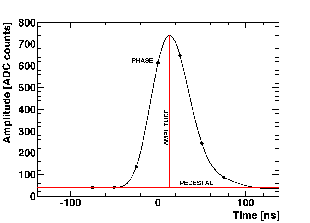
\includegraphics[width=\textwidth]{TileTimingPerformance/Figures/figures_Optimal_Filtering_With_Iterations.pdf}%
    \caption{}
    \label{fig:pulse_shape}
    \end{subfigure}
    \begin{subfigure}{0.49\textwidth}
    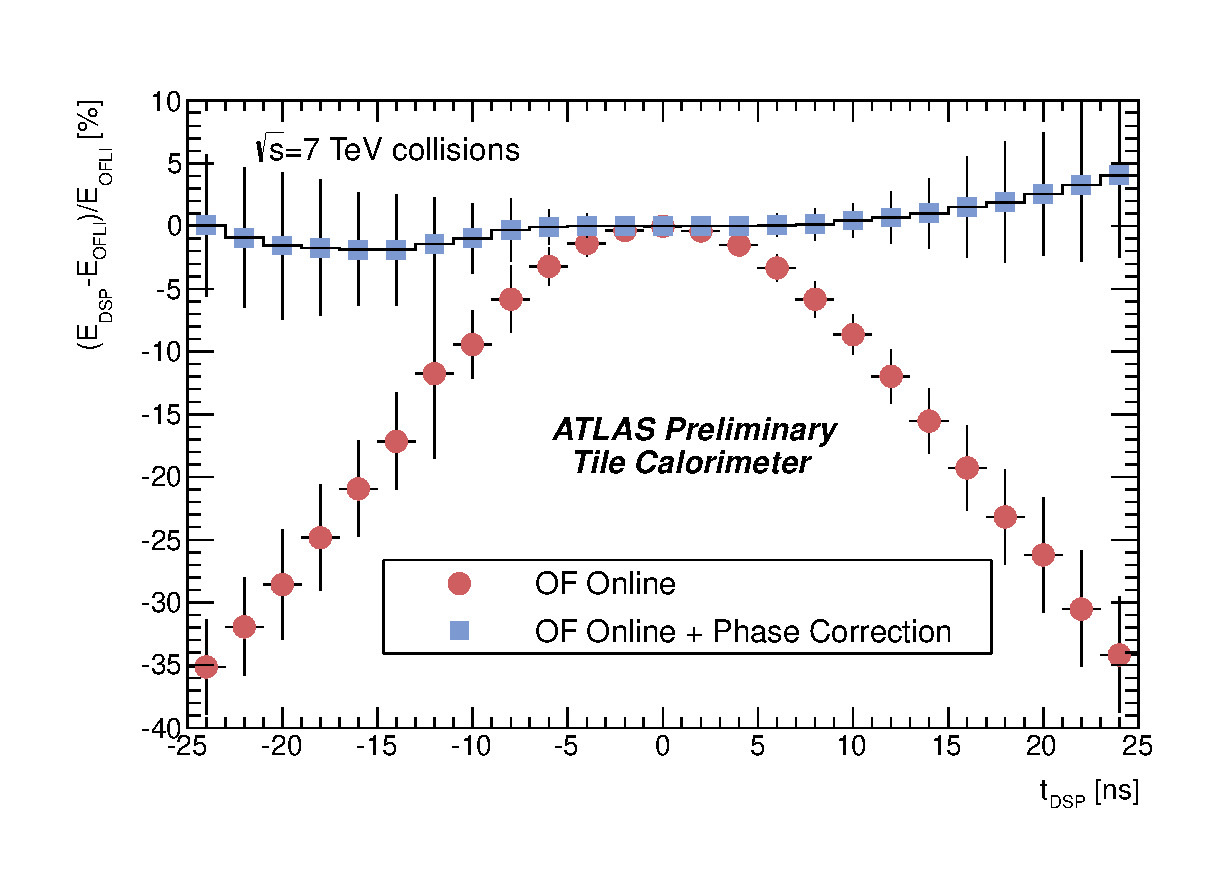
\includegraphics[width=\textwidth]{TileTimingPerformance/Figures/collisions_182284_7TeV_ParabolicProfile_FinalUpdate_140512.eps}
    \caption{}
    \label{fig:pulse_offline}
    \end{subfigure}
  \end{center}
  \caption{(a) Reconstruction of the main characteristics of the pulse from the sampled values: amplitude, arrival phase and baseline level, or pedestal.
    (b) Pulse amplitude reconstructed online with respect to the pulse reconstructed with correct (known) phase, 
    as a function of the cell time ($t_{\rm DSP}$).
    For non-zero phases the
    amplitude as reconstructed online (red points) can be corrected offline (blue squares).
  }
  \label{fig:pulse}
\end{figure}
Figure \ref{fig:pulse_shape} shows an analog signal pulse and the ADC measurement samples, and illustrates the main characteristics of the pulse: amplitude, arrival phase and baseline level, or pedestal.
These are measured using the optimal filtering algorithm \cite{optimal_filtering}.
The phase of the calorimeter signals from \pp\ collisions events is expected to be synchronized with the LHC clock and constant within very small fluctuations due to the longitudinal spread of proton bunches.
The ADC measurement phase can be adjusted to compensate for delays and
time of flight.
After this adjustment all the channels are expected to
have their mean time $\left< t_{\rm channel} \right> = \unit[0]{ns}$.
If the channel mean time is not well adjusted, the reconstructed
amplitude is underestimated as demonstrated in figure~\ref{fig:pulse_offline}.
Although the amplitude can still be corrected offline, the
precision of this additional correction deteriorates with the
phase~\cite{signal_reco_precision}.
In addition, the non-zero $\left< t_{\rm channel} \right>$ affects
the overall time resolution as will be demonstrated in section~\ref{sec:analysis}.

Each cell is read out by two channels, and the cell energy $E_{\rm cell}$ and time
$t_{\rm cell}$, are built using this information:
\begin{eqnarray}
  \label{eq:e_cell}
  E_{\rm cell} & = & E_{{\rm channel} ,1} + E_{ {\rm channel},2} \\
  \label{eq:t_cell}
  t_{\rm cell} & = & (t_{ {\rm channel} ,1} + t_{ {\rm channel} ,2})/2
\end{eqnarray}


The presence of collisions every \unit[50]{ns} and the large read-out window of \unit[150]{ns} lead to a significant fraction of calorimeter cells receiving energies from more than one bunch crossing in the same read-out window, as can be seen in figure~\ref{fig:pileup}.
This has an impact on the reconstruction of the energy deposited in a cell.
A quality factor is computed online for each event and for each calorimeter channel within the trigger latency, based on the compatibility of the sampling with the expected pulse shape.
This allows the identification of calorimeter channels presenting significant contamination from out-of-time \pileup~\cite{pileup_identification}.

\begin{figure}[tb!]
  \begin{center}
    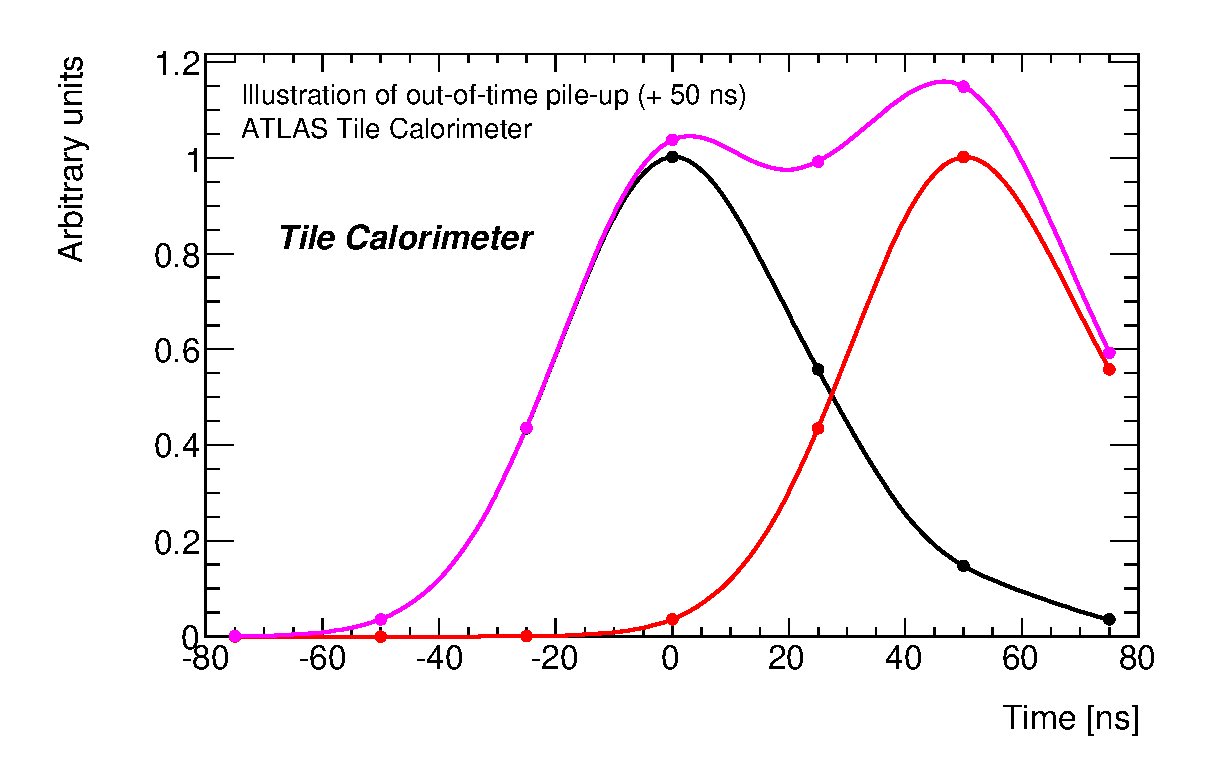
\includegraphics[width=0.6\textwidth]{TileTimingPerformance/Figures/Pileup_Pulses.eps}
  \end{center}
  \caption{Illustration of the effect of out-of-time \pileup. A pulse due to out-of-time \pileup\ (red) overlays a pulse from the collision of interest (black). The resulting signal from the sampling (purple) is significantly distorted with respect to the nominal one.}
  \label{fig:pileup}
\end{figure}

\subsection{Channel timing calibration}
\label{sec:calibration}
The precision
of the signal reconstruction depends on the knowledge of the peak
pulse arrival time with respect to the electronic sampling clock.
%
% The best resolution of the amplitude measurement is
% achieved when the peak is close to the central sample.
The channel time settings is controlled with two programmable delays, referred to as
\textit{dskew2} and \textit{digitizer pipeline} offsets.
%
Two types of calibration are used to calculate these programmable
delays and residual channel mean times: laser calibration and calibration with splash events.
A third method based on data from collision events can be used to monitor the stability and correct deviations.

In 2008 the cell times were synchronized to a single reference channel in every partition using the laser calibration system.
Inter-calibration between partitions was performed in 2008 and 2010 using splash events.

\subsubsection{Laser calibration}
In order to calibrate and monitor the response of the PMTs an integrated laser system is used \cite{timing_laser}.
Laser pulses with a wavelength of \unit[532]{nm} and a pulse width of \unit[15]{ns} from a single laser source are distributed directly into each PMT via a chain of optical fibers.
A \textit{laser run} corresponds to a set of TileCal data taken while the laser is pulsing.
A laser run used for timing analysis normally contains between 3000 and 10000 events or triggers, which is the number of laser pulses sent to each PMT.
From the observed $\left< t_{\rm channel} \right>$ values in a laser run,
one can derive appropriate time corrections, so that
$\left< t_{\rm channel} \right>$ is made uniform over the entire
calorimeter for a simultaneous energy deposition.


\subsubsection{Splash events}
LHC can operate with one beam only to generate splash events.
In such events protons from the beam collide with collimators placed at \unit[140]{m} from the nominal interaction point and produce a very large number of secondary particles, reaching the detector nearly parallel to the beam axis and depositing a large amount of energy in the whole calorimeter.
After correcting for the difference in time of flight with respect to the interaction point, these events can be used to extract the absolute calibration for the timing constants of each channel~\cite{splash_calib_summary,splash_calib_public_plot}.

\subsubsection{Calibration with collision events}
Due to the large \xsec, jets from collision events can be used to compute the channels' mean time during data taking periods. Deviations in the channel offset or digitizer offset constants can be corrected in order to retain the best possible calibration. Channels with problematic time reconstruction are identified and flagged to avoid the usage of the measured time for energy corrections. This calibration can also be performed with muons from collision events, and will be discussed in the following.

\section{Object definition and event selection}
\label{sec:selection}
The analysis presented here is performed with isolated muons
in the 2011 collision data at the \com\ energy of $\sqrt{s}=\unit[7]{\TeV}$ and $\unit[50]{ns}$ bunch crossing
separation.
Data from three runs belonging to Period K in the 2011 dataset are used.
The datasets correspond to a total integrated luminosity of $\unit[127.2]{pb^{-1}}$.
The object definition and event selection is briefly described
in the following sections.
%and are processed using a customized version of the package \texttt{TileAnalysis}.

\subsection{Muons}
From the variety of muon reconstruction schemes, combined muons are used,
which are reconstructed using information from both
the muon spectrometer and the inner detector
% . The muons used in this study are combined muons as reconstructed 
by Muid~\cite{muon_id}.
The algorithm takes inner detector tracks and muon spectrometer tracks and
combines them via a $\chi^2$ minimization scheme.
It incorporates
detector response functions and accounts for possible scattering of
the muon between the inner detector and the muon spectrometer to give
realistic results.

The following selection cuts are imposed on the muon candidates:
\begin{itemize}
\item Muon momentum $p>\unit[3]{GeV}$.
\item Muon transverse momentum $p_T>\unit[1]{GeV}$.
\item Pseudorapidity of the reconstructed muon track $|\eta_{\mathrm{track}} | < 2$.
\item At least 6 hits in the SCT and 1 hit in the pixel detectors.
\item Tracking and calorimeter isolation is required in a cone $\Delta R < 0.4$ around
    the muon excluding the muon itself: $p_T^{0.4} <\unit[2]{GeV}$ and $E_T^{0.4} <\unit[2]{GeV}$.
\end{itemize}

\subsection{Calorimeter cells}
The whole volume of the Tile calorimeter is studied, using both the long and the extended barrel.
  Special TileCal cells
such as gap/crack cells and  
minimum bias trigger scintillators (MBTS) are removed and will not be
further considered in this analysis.

For each event, all cells inside a cone
of $\Delta R < 0.2$ around the muon track, as defined in
equation~\ref{eq:deltaR_tilecal}, are considered:
\begin{equation}\label{eq:deltaR_tilecal}
	\Delta R = \sqrt{\left( \phi_{\mathrm{track}} - \phi_{\rm cell~center}\right)^2+\left( \eta_{\mathrm{track}} - \eta_{\rm cell~center}\right)^2}~,
\end{equation}
where $\eta_{\mathrm{track}}$ and $\phi_{\mathrm{track}}$ are the reconstructed muon
track coordinates extrapolated to the corresponding calorimeter layer.

Further selection requirements are applied on the calorimeter cells
\begin{itemize}
\item The cell is not flagged as ``bad cell'' and none of the associated
  PMTs is masked. A cell can be flagged as bad due to read-out problems or excessive noise.
\item The cell is crossed by a muon track.
\item The energy deposited in the cell is greater than the noise
  threshold: ${E_{\rm cell} > \unit[540]{\mev}}$.
% \item The cell time $t_{\rm cell}$ has been correctly
%   reconstructed. Normally, the cell time is considered as a straight
%   average of the corresponding channel times $t_{\rm channel}$, provided
%   both of them are correctly reconstructed. Note that for small
%   signals the time is fixed $t_{\rm channel} \equiv 0$ to avoid large RMS
%   in the reconstructed energy.
\item The path length inside the cell is at least 30\% of the path
    length in the corresponding longitudinal layer.
\item The difference between the cell time $t_{\rm cell}$ and the mean
    time in that cell is less than
    \unit[15]{ns}, $| t_{\rm cell} - \left< t_{\rm cell} \right>| <
    \unit[15]{ns}$.
\end{itemize}

\subsection{Outlier removal}
As mentioned in section~\ref{sec:calibration}, the time calibration of
the channels is performed in order to obtain $\left< t_{\rm channel}
\right>=\unit[0]{ns}$ for each channel, and consequently the mean cell time
$\left< t_{\rm cell} \right>=\unit[0]{ns}$ in each cell.
However, miscalibrations,
hardware problems or other effects can introduce imperfections in the
calibration and therefore $\left< t_{\rm channel}
\right>\neq\unit[0]{ns}$. 
In cases where the miscalibration is severe the cells are considered
outliers.
Those cells are removed from the analysis
as their presence affects refined studies such as the detector
intrinsic resolution.
Two issues are addressed in this section which may lead to the removal of affected cells: outlier channels and unstable digitizers.

Due to a variety of reasons, the miscalibration of the channels can
lead to  $\left< t_{\rm channel} \right> \neq \unit[0]{ns}$.
Using jets from collision events, the mean time of each channel can be computed.
Channels with $| \left< t_{\rm channel} \right> | > \unit[5]{ns}$ are flagged as outliers.
Cells with at least one outlier channel are removed from this analysis.
%
%This cut was applied in order to remove cells which were seriously miscalibrated.

An unresolved problem of the Tile calorimeter during the 2011 data taking was
the instability of digitizers' time settings.
Some digitizers can lose their time settings, resulting in
a shift in the digitizer time as can be seen in figure
\ref{fig:jump}.
These shifts can be identified using laser calibration events in empty orbits.
All the cells with at least one channel reconstructed by an affected digitizer are removed from the analysis.

\begin{figure}[tb!]
  \begin{center}
      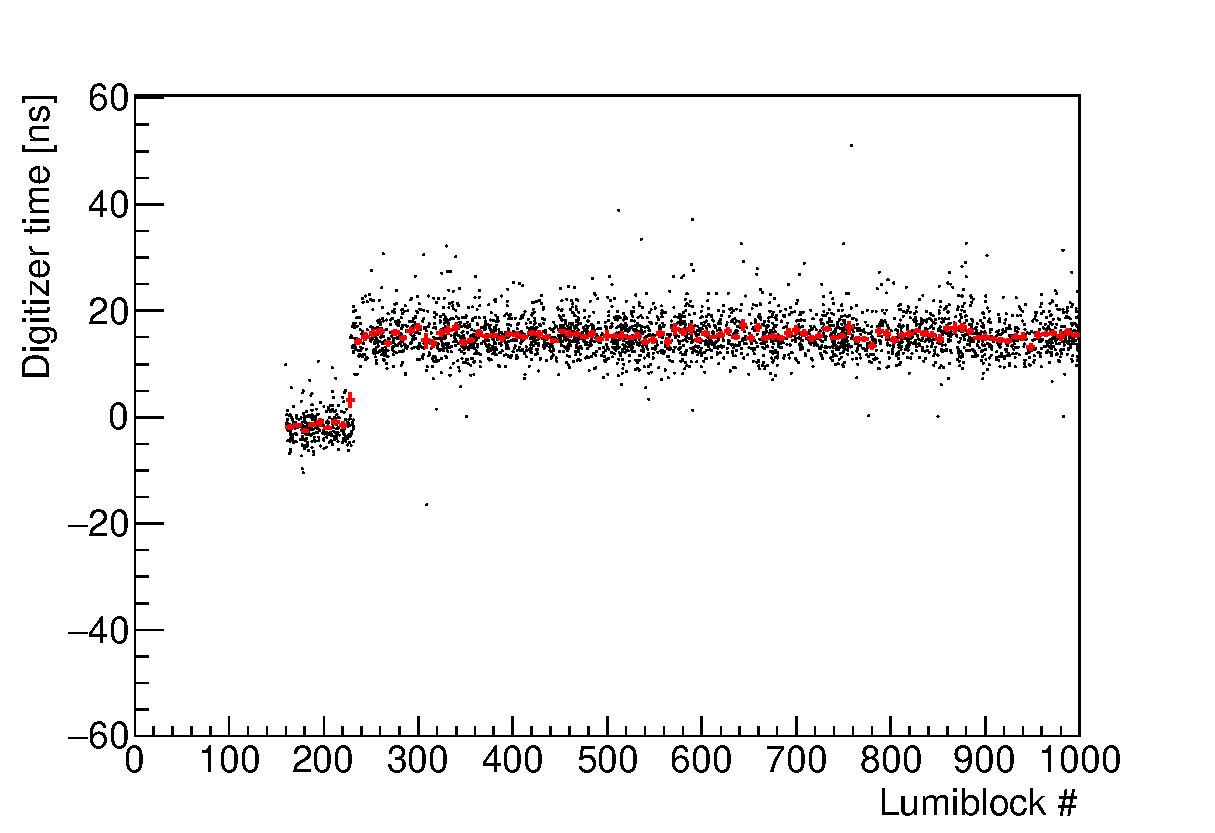
\includegraphics[width=0.6\textwidth]{TileTimingPerformance/Figures/jump.eps}
      \label{fig:digi_lumi}
  \end{center}
  \caption{Example of a timing shift in digitizer 6 of EBC module 22,
    during run 187014. Red markers show the average over 10 lumiblocks. The mean digitizer time shows a clear jump around lumiblock 250.}
  \label{fig:jump}
\end{figure}

In total, 123 cells were removed from the analysis,
representing approximately \unit[2.5]{\%} of all TileCal cells.


\section{Analysis}
\label{sec:analysis}
The time measurement is usually characterized by the
dependence of the time resolution on energy.
However, as it will be demonstrated, this parameterization does not provide an accurate modeling of the
observed time resolution, which hints at the existence of other sources or
effects affecting the timing.
The inclusion of further observables and their effect is studied
in each calorimeter sample and partition, and integrated over the
whole calorimeter.

One important aspect in the response of the calorimeter is the nature
of the particles depositing the energy.
Whereas hadronic particles
create showers whose energy is almost entirely deposited in the
calorimeter, muons behave mostly as minimum ionizing particles.
Muons of selected momentum leave in the calorimeter an amount of energy
roughly proportional to the traversed path length.
This behavior
introduces a strong correlation between the measured energy and
observables that, given the geometry of the calorimeter, could be
correlated to the path length.
Some examples of these observables are
the size of the cell, the distance to the interaction point or the
position in $\eta$, all of which scale roughly with the path length.

%A real dependence in the investigated observable will yield the same
%behavior in all the samples, whereas a residual dependence, arising
%from its correlation to a different observable, will result in
%different patterns across the different calorimeter samples. A common
%analytic dependence across samples, but with different values, is most
%probably pointing to additional observables affecting the
%timing. Additionally to the analysis of the resolution, the mean time
%dependence with each observable is studied.

\subsection{Energy dependence}
\label{subsec:energy}
As the first step, the timing performance is investigated as a function
of the cell energy.
The time resolution of the detector is parameterized by:
\begin{equation}
  \label{eq:timing_resolution_vs_energy}
  \sigma = \sqrt{{p_0}^2+\bigg(\frac{p_1}{\sqrt{E}}\bigg)^2+\bigg(\frac{p_2}{E}\bigg)^2}~.
\end{equation}
This parameterization accounts for the electronic noise, proportional to
$1/E$, a statistical term $1/\sqrt{E}$, and a constant term that
accounts for miscalibrations and other detector imperfections.
A priori, no dependence of the mean time with energy is expected.

The dependence of the mean time with the cell energy is shown in figure~\ref{fig:mean_vs_energy}.
A clear bias towards negative times is observed, and a flat dependence with energy.
This bias will be further investigated and explained in section~\ref{subsubsec:bias_in_timing}.

As can be seen in figure~\ref{fig:resolution_vs_energy}, the time resolution is qualitatively well
described by equation~\ref{eq:timing_resolution_vs_energy}.
The result of the fit is shown in table~\ref{tab:fit_result}.
The value of $\chi^2$, corresponding to a probability of $\sim 10^{-10}$, suggests that further
observables are needed for an improved description of the
resolution.


\begin{table}
  \begin{center}
    \begin{tabular}{ c  c l }
      \toprule
      \toprule
      $\chi^2/$ndof & 83.78/19 & \\ 
      $p_0$ & $0.75 \pm 0.01$ & ns \\ 
      $p_1$ & $1.38 \pm 0.02$ & ns $\GeV^{1/2}$ \\ 
      $p_2$ & $0.76 \pm 0.02$ & ns $\GeV$ \\ 
      \bottomrule
      \bottomrule
    \end{tabular} 
    \caption{Time resolution with isolated muons, result of the fit to
      the resolution function~(\ref{eq:timing_resolution_vs_energy}).} 
    \label{tab:fit_result}
  \end{center}
\end{table}

 
\begin{figure}[!tb]
  \begin{center}
    \begin{subfigure}{0.49\textwidth}
      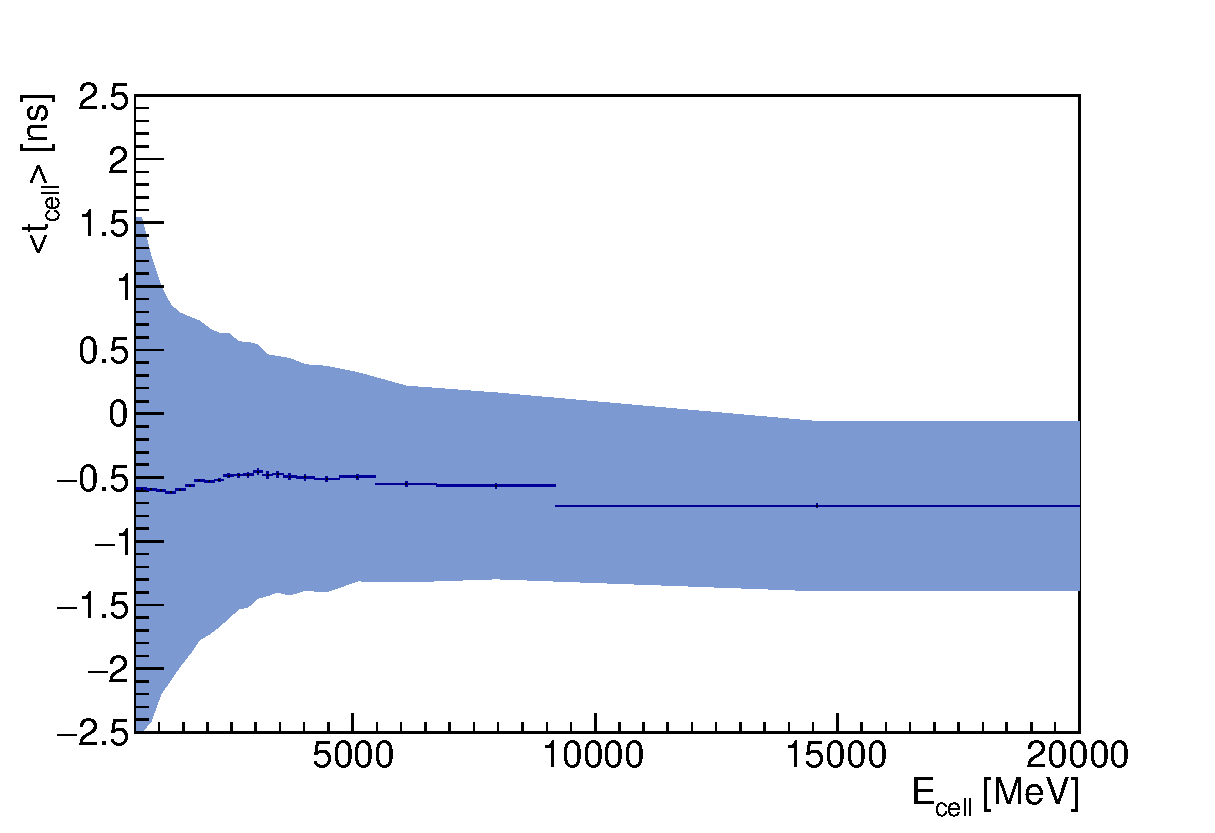
\includegraphics[width=\textwidth]{TileTimingPerformance/Figures/e_mean.eps}
      \caption{}
      \label{fig:mean_vs_energy}
    \end{subfigure}
    \begin{subfigure}{0.49\textwidth}
      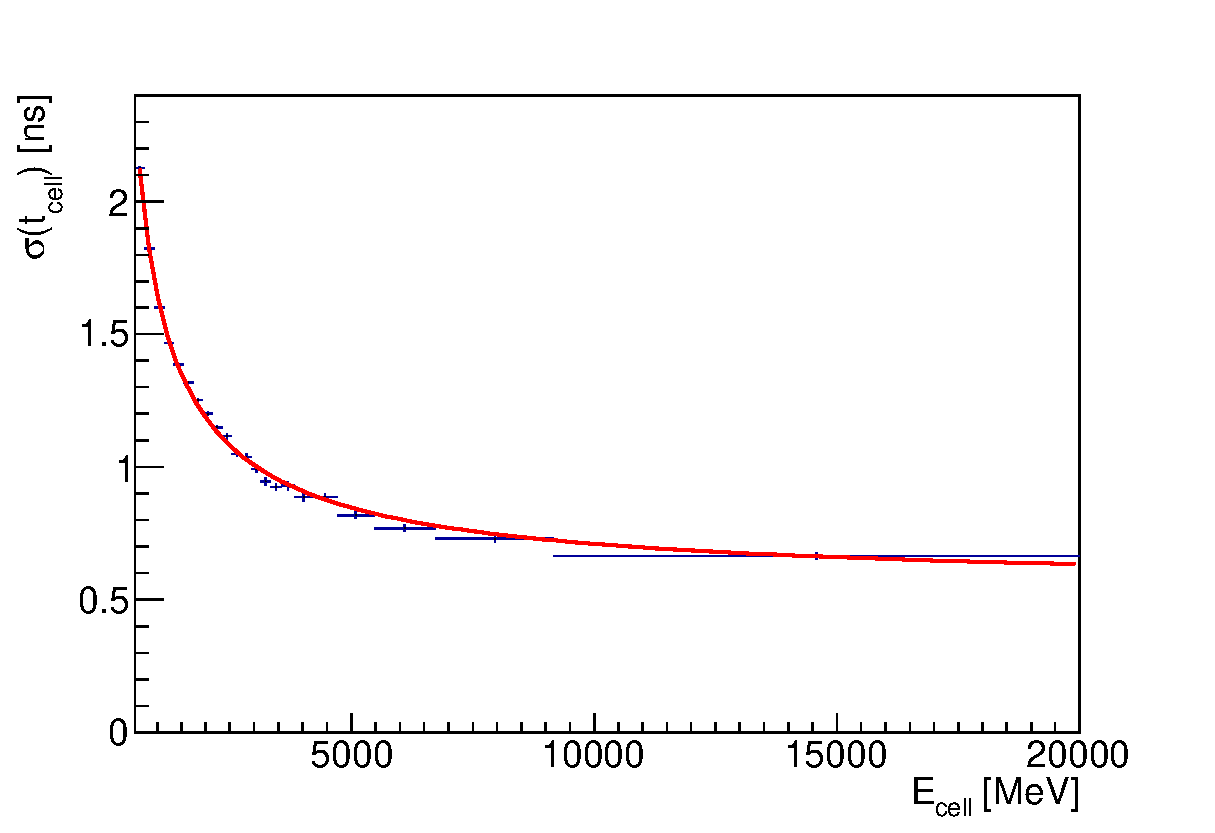
\includegraphics[width=\textwidth]{TileTimingPerformance/Figures/e_res.eps}
    \caption{}
    \label{fig:resolution_vs_energy}
    \end{subfigure}
  \end{center}
  \caption{(a) Mean cell time and (b) resolution dependence with
    energy. Error bars represent the statistical errors, the shaded area represents the expected resolution for the given energy.}
  \label{fig:e}
\end{figure}

A decomposition of the contribution of the
different samples is performed and shown in figure~\ref{fig:e_split}.
The resolution dependence in all samples
resembles equation~\ref{eq:timing_resolution_vs_energy}, while 
the different values of the fitted parameters highlight the need for other observables to reach a correct
description.
The mean time however, shows a clear variation across
samples.
%This dependence will be addressed in section~\ref{subsubsec:bias_in_timing}.

 
\begin{figure}[tb!]
  \begin{center}
    \begin{subfigure}{0.49\textwidth}
      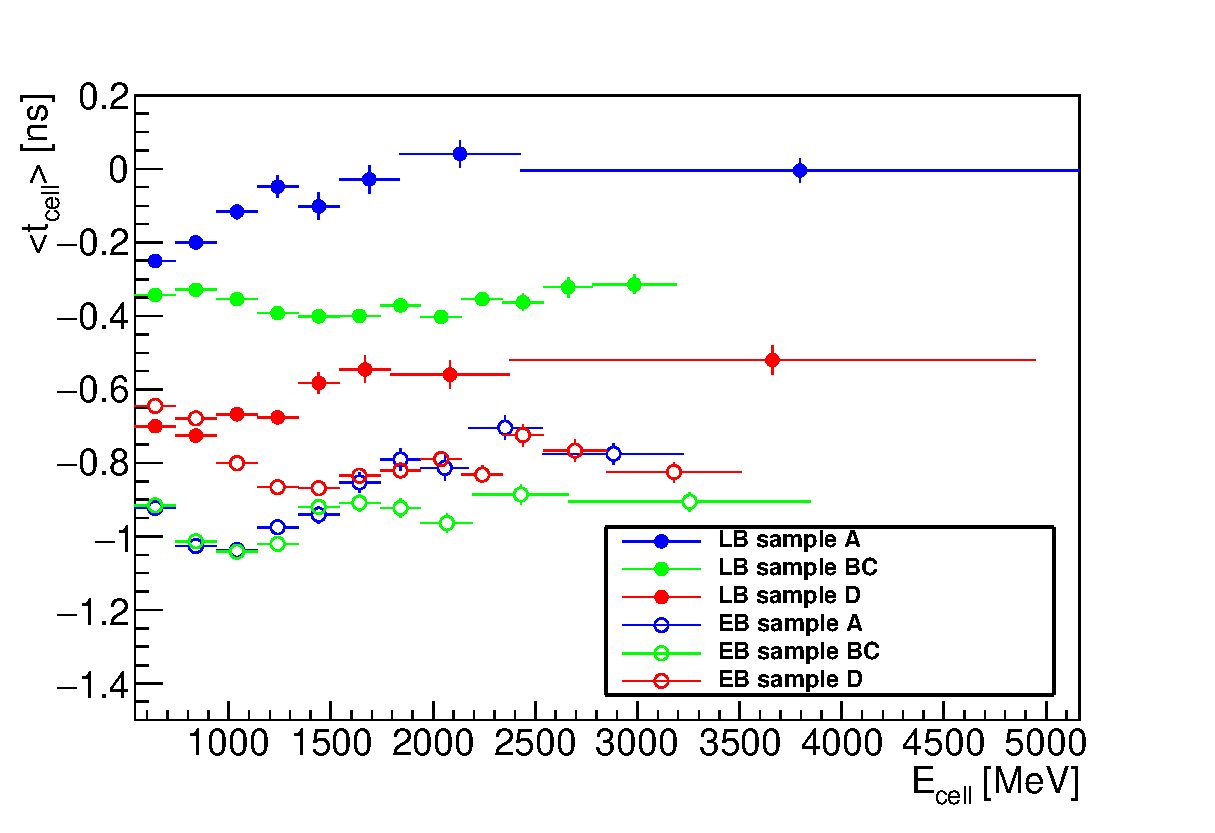
\includegraphics[width=\textwidth]{TileTimingPerformance/Figures/e_mean_split.eps}
      \caption{}
      \label{fig:mean_vs_energy_split}
    \end{subfigure}
    \begin{subfigure}{0.49\textwidth}
      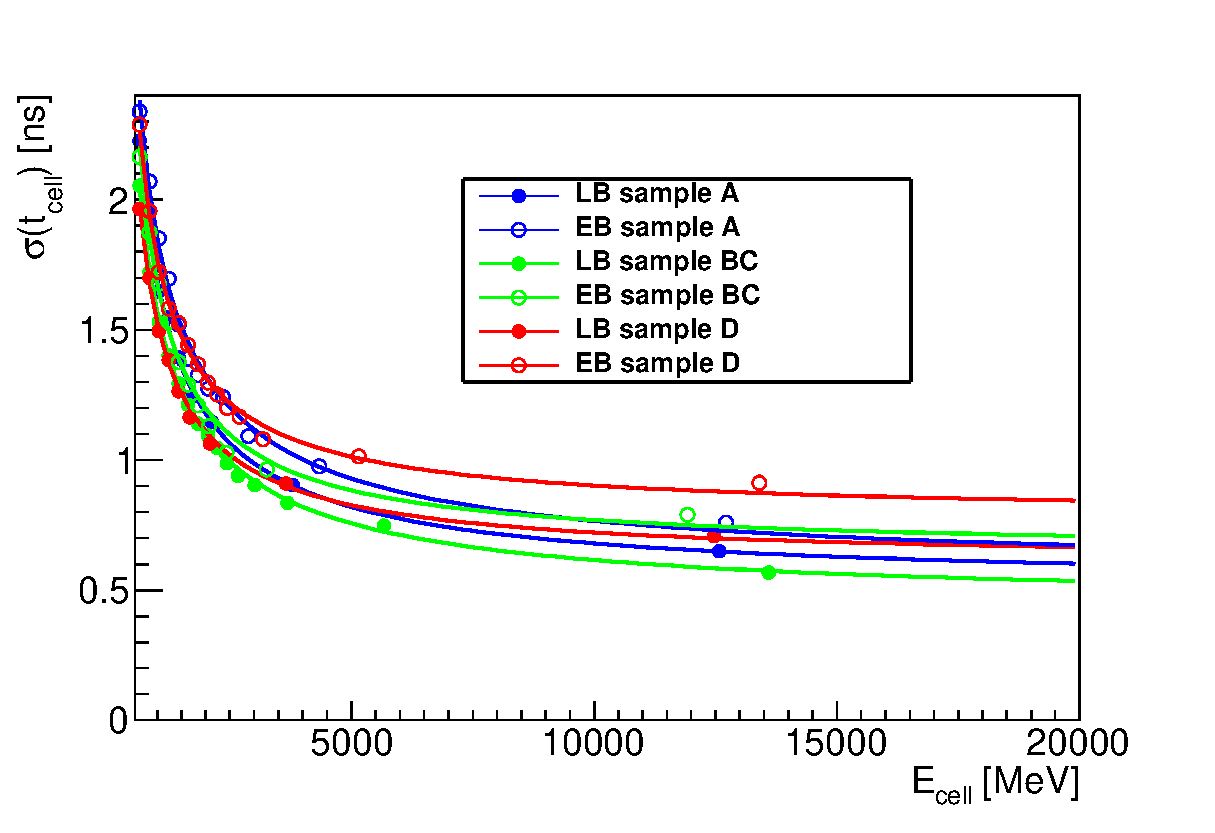
\includegraphics[width=\textwidth]{TileTimingPerformance/Figures/e_res_split.eps}
    \caption{}
    \label{fig:resolution_vs_energy_split}
    \end{subfigure}
  \end{center}
  \caption{(a) Mean cell time and (b) time resolution as a function of
    energy in the individual calorimeter samples.}
  \label{fig:e_split}
\end{figure}

\subsection{Distance to the interaction point}
\label{subsec:distance}
It can be argued that there is no reason to expect variations in resolution or a mean time dependence with the distance to the interaction point, since the timing of all cells has been corrected for the expected time of flight.
However, multiple scattering or other geometrical and detector effects correlated with the distance could affect the timing performance.
Since the mean energy deposition depends on the geometry of the cell, 
the resolution is studied as the difference to the expected resolution given the mean value of the energy in that cell.

Figure~\ref{fig:distance} shows the results for the dependence with
distance, from which two conclusions can be drawn.
First, there is an obvious
dependence of the mean time with distance, with cells further away
from the interaction point reporting a lower value of the mean time.
%This will be discussed in section~\ref{subsubsec:bias_in_timing}.
Additionally, analyzing the difference in resolution, a pattern 
becomes apparent:
the resolution degrades for cells in the most forward region
of each sample, and improves for samples further away from the
beam pipe.
A more visually intuitive representation of this pattern
can be observed in figure~\ref{fig:map_diff}.
A possible explanation
for this effect will be given in sections~\ref{sec:pathdiff}
and~\ref{sec:pileup}.
\begin{figure}[tb!]
  \begin{center}
    \begin{subfigure}{0.49\textwidth}
      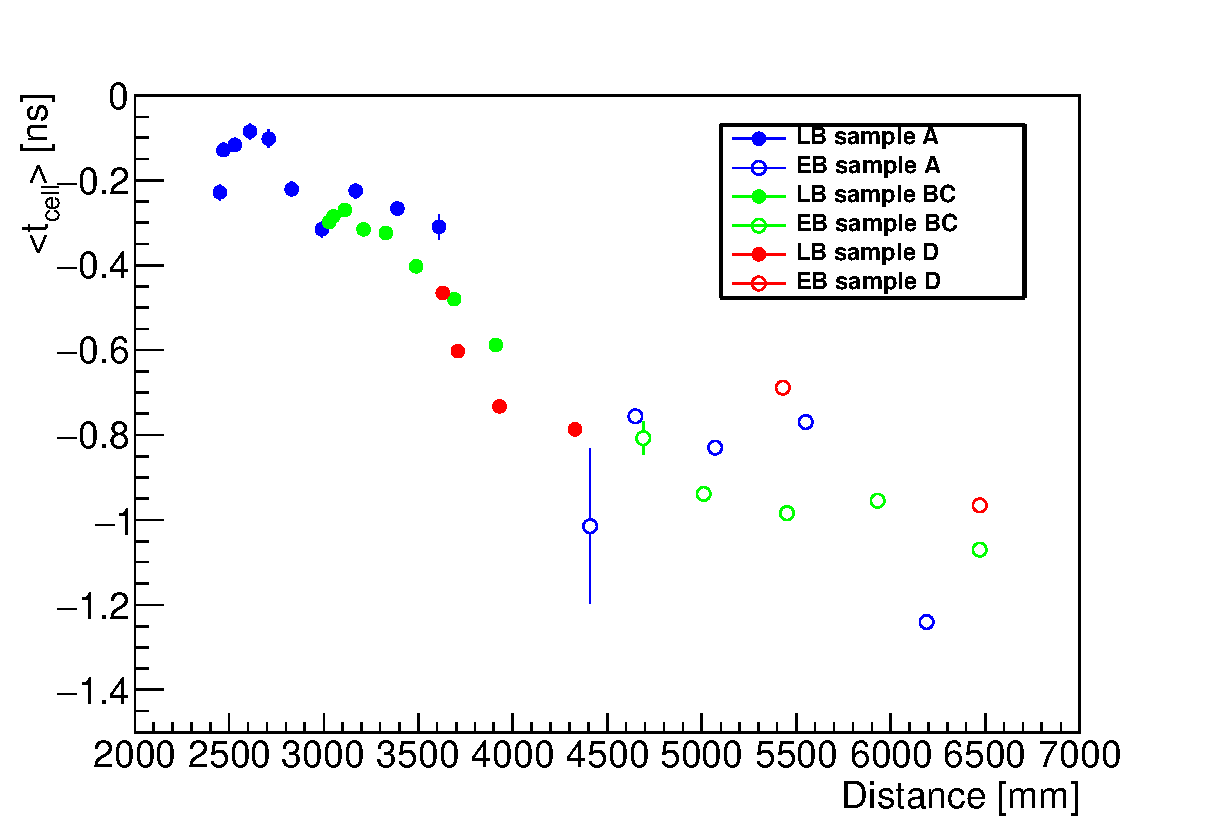
\includegraphics[width=\textwidth]{TileTimingPerformance/Figures/distance_mean.eps}
      \caption{}
      \label{fig:distance_mean}
    \end{subfigure}
    \begin{subfigure}{0.49\textwidth}
      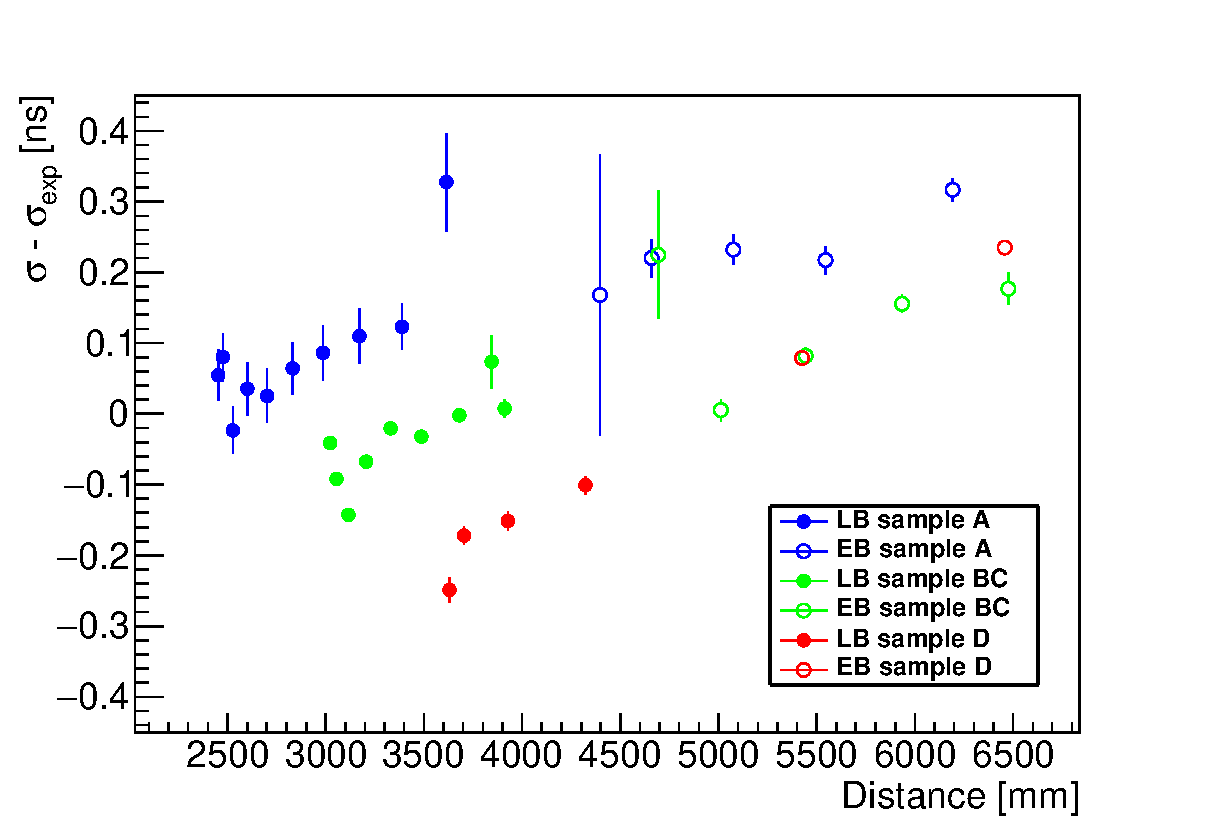
\includegraphics[width=\textwidth]{TileTimingPerformance/Figures/distance_res.eps}
      \caption{}
    \label{fig:distance_res}
    \end{subfigure}
  \end{center}
  \caption{(a) Mean cell time and (b) difference in the time resolution to the 
  expected value given the mean value of the energy deposition, 
    as a function of the cell distance to the interaction point and averaged over cell energy.
  }
  \label{fig:distance}
\end{figure}

\begin{figure}[tb!]
  \begin{center}
    \hspace{0.5cm}
    \begin{overpic}[width=0.9\textwidth]{TileTimingPerformance/Figures/mapnewcut.pdf}
       \put (20,24) {LB}
       \put (70,24) {EB}
       \put (-4,1) {A}
       \put (-6,10) {BC}
       \put (-4,19) {D}
     \end{overpic}
    %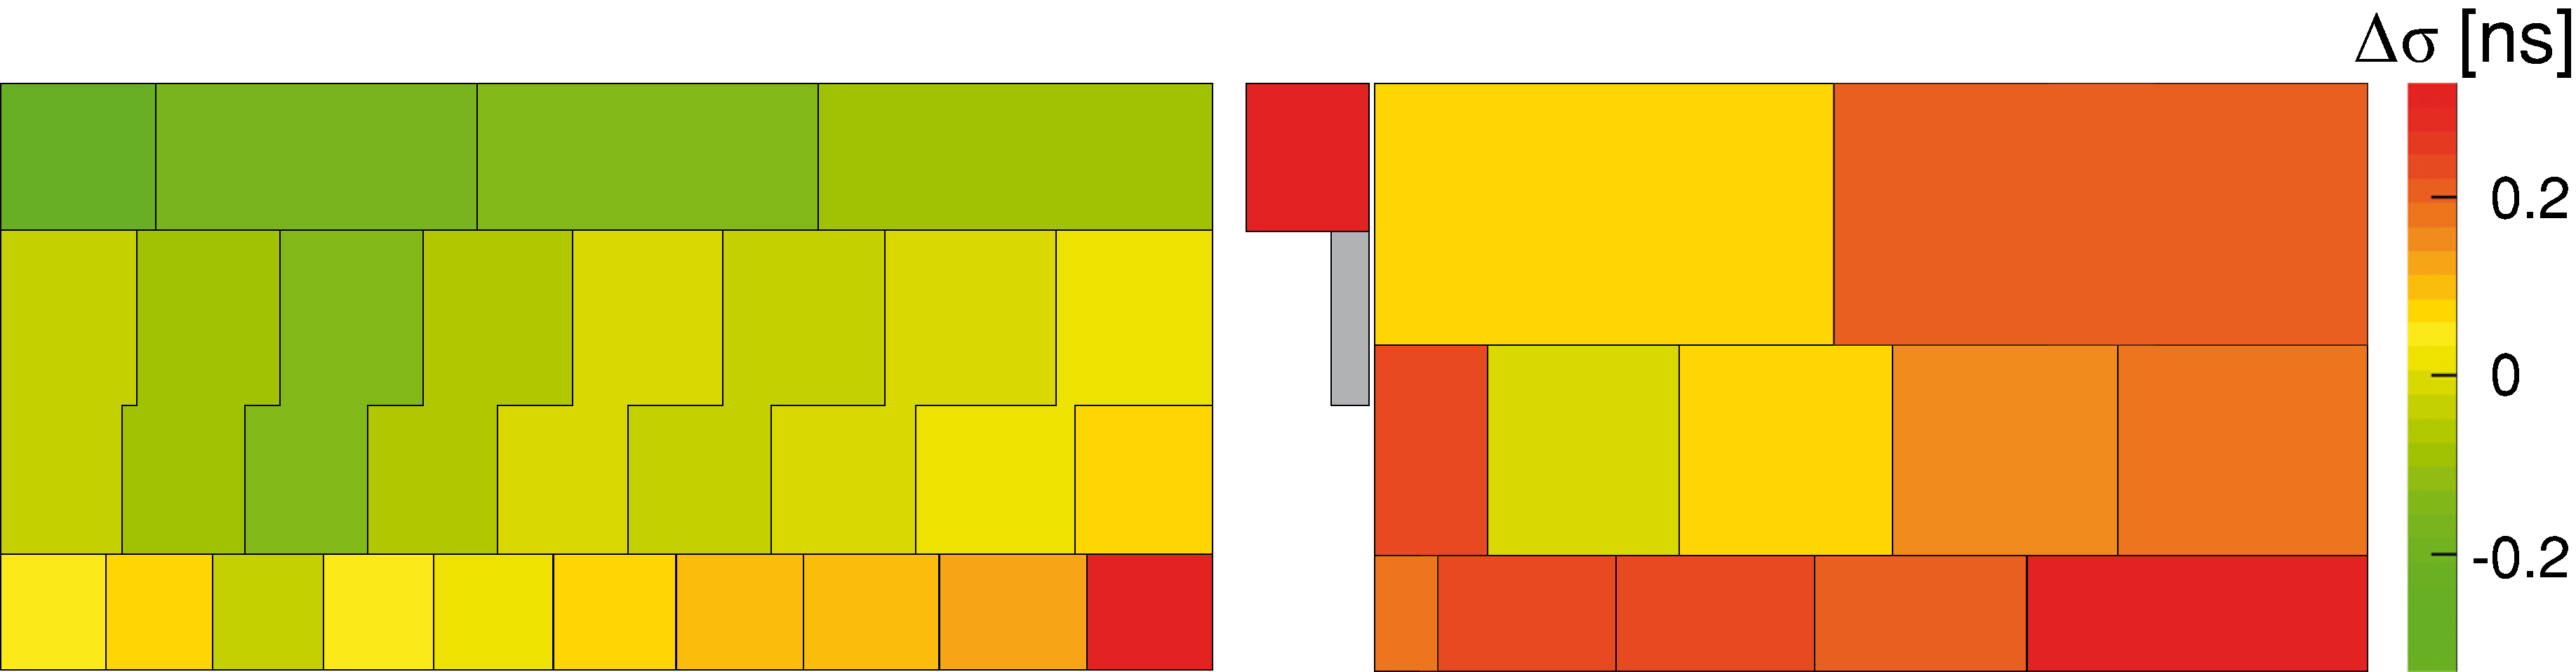
\includegraphics[width=0.90\textwidth]{TileTimingPerformance/Figures/mapnewcut.pdf}
  \end{center}
  \caption{Difference between measured resolution and expected resolution from its energy deposition, averaged over cell energy.}
  \label{fig:map_diff}
\end{figure}

\subsubsection{Bias in timing}
\label{subsubsec:bias_in_timing}
Focusing again on the mean time dependence with distance, a proper explanation is needed.
The aforementioned multiple scattering effect would result in a higher value of the mean time for distant cells, whereas the opposite effect is seen.

Since no obvious physical effect can account for an increase in the speed of the muon while it traverses the calorimeter, a different approach has to be considered.
This effect can be explained if the calibration of the cell's time is biased, with values increasing with distance.
Since the calibration of the cell time is performed with splash and laser events, there should be no reason for this bias.
However, further  corrections are performed based on studies involving jets from collision events.
The development of the hadronic shower across the calorimeter is slower than the muons' speed~\cite{timingpublicplots}.
Therefore, all the tuning that is performed using jet data will introduce a bias towards higher time values for distant cells.
At least two sources of bias can be identified:
\begin{itemize}
  \item Digitizer offsets are corrected with data from jet events in order to stay as close as possible to  $\left< t_{\rm channel} \right> = \unit[0]{ns}$.
  \item 
  The spotting and removing of outliers is also performed based on jet studies, thus removing more easily cells with high timing and leaving those with lower timing.
\end{itemize}

For the rest of the analysis, the timing of each cell is corrected to its mean time.
Therefore imposing a perfectly in-time detector.
This will improve artificially the resolution but it will as well allow for the study of the mean time dependence in observables that are cell-independent, e.g.
the position of the track respect to the cell center.

\subsection{Path difference}\label{sec:pathdiff}

It has been already mentioned that the mean time of the cells is corrected for the time of flight.
However, this correction is computed for the cell center, and the difference in path distance for muons that don't cross the cell at its center can be non-negligible, especially for the larger cells.
As a reference, the dimensions of the largest TileCal cell (D6) are $\unit[680]{mm} \times \unit[1369]{mm}$, and it takes a muon \unit[4]{ns} to traverse it.

A new observable is studied, measuring the difference in path with respect to the center of the cell, as defined in equation~\ref{eq:pathdiff_def}.
A linear dependence is expected, with a slope equal to the speed of the muons, $\approx c$.

\begin{equation}
  \label{eq:pathdiff_def}
  \Delta_{\rm path} = \left( D_{ip} + D_{op} \right) / 2 - D_{cc}~,
\end{equation}
where $D_p$ is the distance from the interaction point to point $p$, and $ip$, $op$, $cc$ are the incoming impact point, outgoing impact point and cell center respectively.

Figure \ref{fig:distancediff_mean}, shows the dependence in this new observable superimposed with the expected slope.
There is a clear deviation at extreme values that can be explained by accounting for the additional path difference of the light in the wavelength-shifting fibers, according to the impact point of the muon, as defined in equation~\ref{eq:fiberdiff_def}.
The energy deposited by muons impacting in the upper half of the cell has less fiber length to traverse before reaching the PMT.

\begin{equation}
  \label{eq:fiberdiff_def}
  \Delta_{\rm fiber} = \left( R_{ip} + R_{op} \right) / 2 - R_{cc}~,
\end{equation}
where $R_p$ is the distance from the beam line to point $p$, and $ip$, $op$, $cc$ are the incoming impact point, outgoing impact point and cell center respectively.

After introducing a correction for the difference in fiber length, the mean time behaves as expected, as can be seen in figure \ref{fig:distancediff_corr_mean}.
This variation of the mean time is especially important for large cells or cells with high $|\eta|$; therefore, this effect is one of the sources of the resolution pattern seen in figure~\ref{fig:map_diff}.

\begin{figure}[tb!]
  \begin{center}
    \begin{subfigure}{0.49\textwidth}
      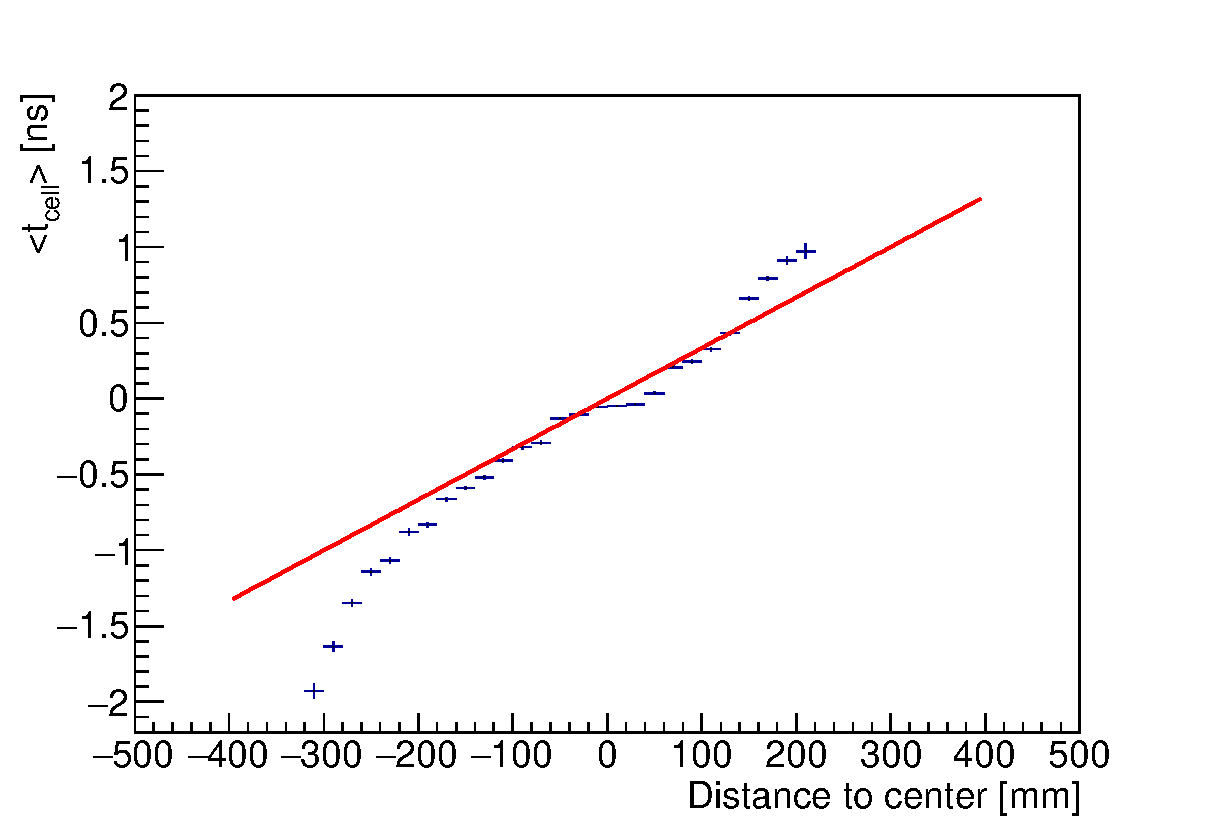
\includegraphics[width=\textwidth]{TileTimingPerformance/Figures/distancediff_mean.eps}
      \caption{}
      \label{fig:distancediff_mean}
    \end{subfigure}
    \begin{subfigure}{0.49\textwidth}
      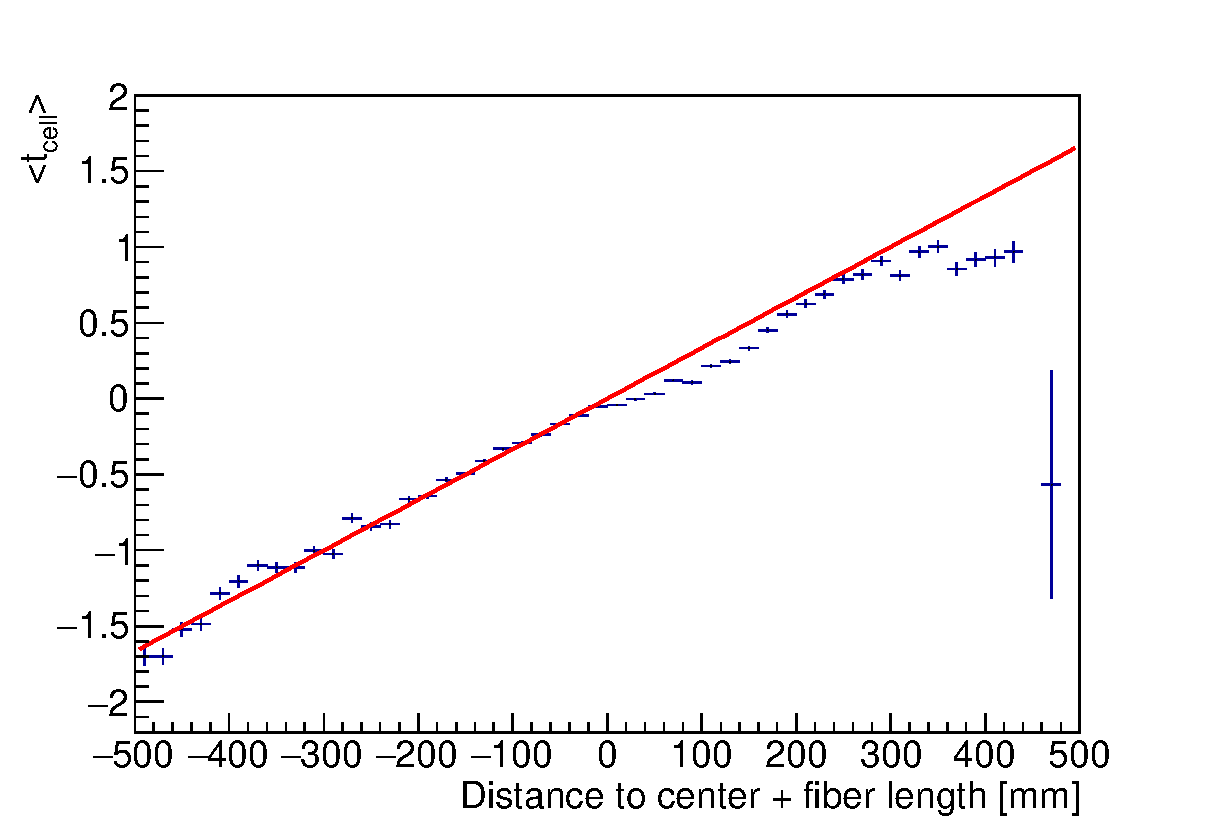
\includegraphics[width=\textwidth]{TileTimingPerformance/Figures/distancediff_corr_mean.eps}
      \caption{}
      \label{fig:distancediff_corr_mean}
    \end{subfigure}
%    \begin{subfigure}{0.49\textwidth}
%      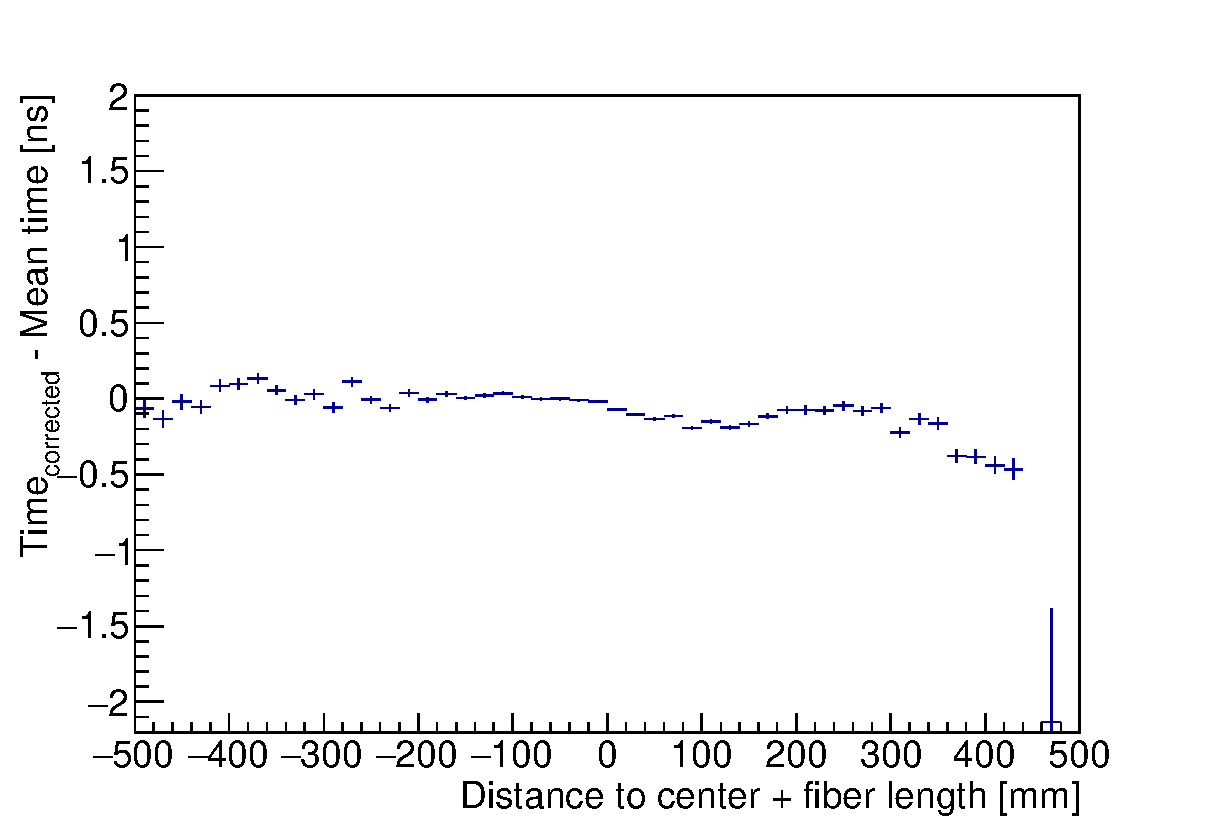
\includegraphics[width=\textwidth]{TileTimingPerformance/Figures/distancediff_corr_mean_flat.eps}
%      \caption{Time spectra after introducing the correction for distance and fiber length difference}
%      \label{fig:distancediff_corr_mean_flat}
%    \end{subfigure}
  \end{center}
  \caption{Mean cell time respect to the distance to the cell center (a) before and (b) after correcting for the difference in fiber length.}
  \label{fig:distancediff}
\end{figure}

The impact of this correction on the overall calorimeter resolution is hardly noticeable, but it improves the resolution of the D layer of the EB, bringing it closer to the resolution of the other samples.

%\begin{figure}[tb!]
%  \begin{center}
%    \begin{subfigure}{0.49\textwidth}
%      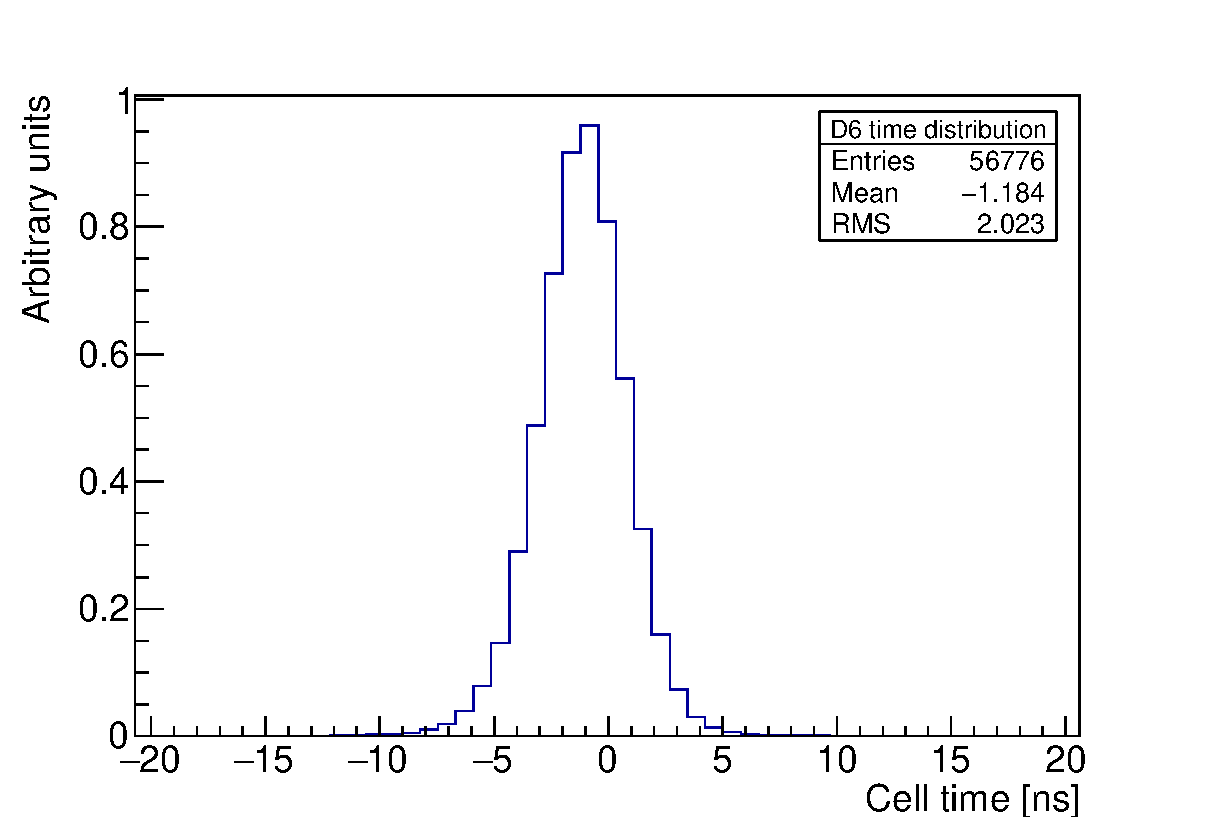
\includegraphics[width=\textwidth]{TileTimingPerformance/Figures/before.eps}
%      \caption{}
%      \label{fig:before}
%    \end{subfigure}
%    \begin{subfigure}{0.49\textwidth}
%      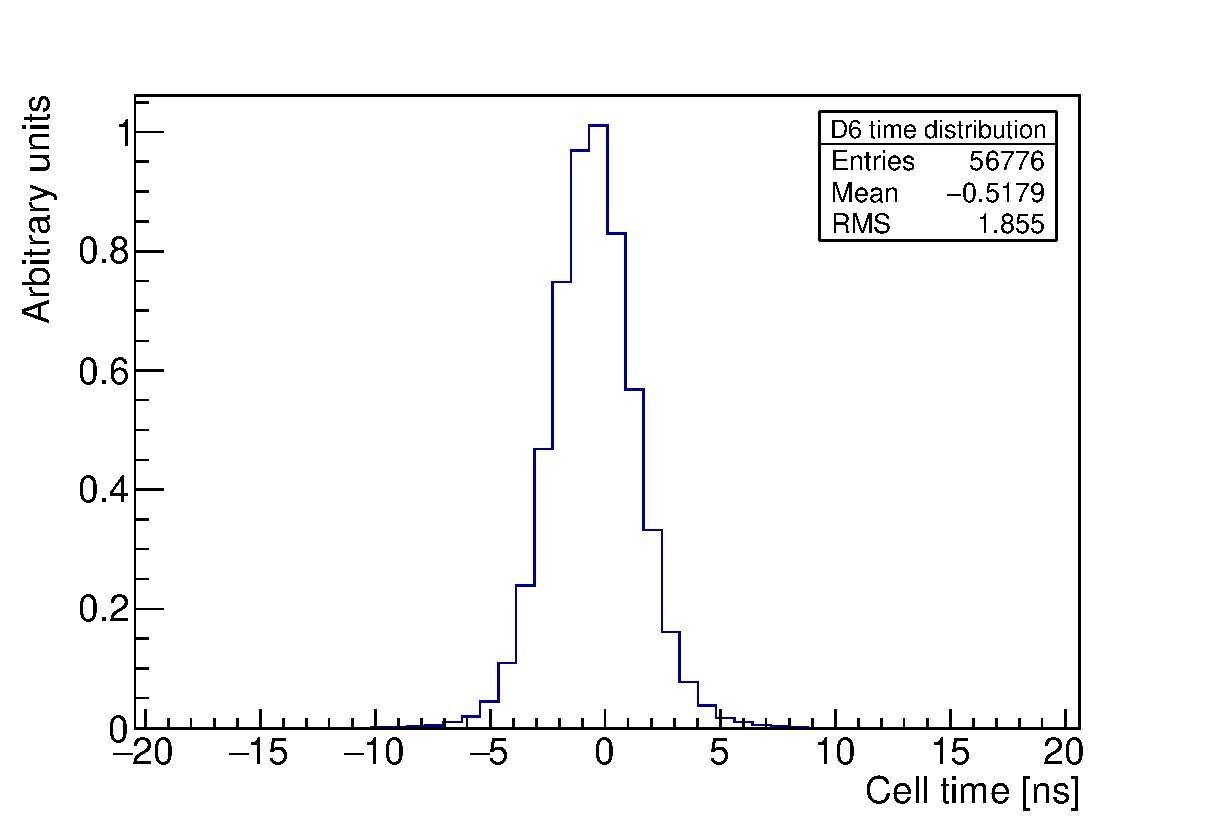
\includegraphics[width=\textwidth]{TileTimingPerformance/Figures/after.eps}
%      \caption{}
%      \label{fig:after}
%    \end{subfigure}
%  \end{center}
%  \caption{(a) Time distribution before and (b) after correcting for the fiber and path difference.}
%  \label{fig:D6_time}
%\end{figure}



\subsection{Energy dependence revisited}
After the analysis of these observables, an updated study of the
energy dependence can be performed.
The changes introduced with respect to the first analysis are:
\begin{itemize}
	\item All cells are corrected to their mean time.
	\item The measured time has been corrected for the
          time of flight difference with respect to the center of the cell, and the time due to the difference in fiber length.
\end{itemize}

After introducing these changes the % energy 
time resolution 
analysis can be repeated.
The result of the fit can be seen in figure
\ref{fig:res_comp} and the fitted parameters are shown in table \ref{tab:compare}.
The fit without corrections is displayed superimposed for comparison.
The biggest improvement in the resolution comes from the correction of the time to the mean time of the cell.

It's noteworthy that although the mean time correction does improve the resolution, it doesn't improve the $\chi^2$ of the fit.
After applying the path difference correction a great improvement in the $\chi^2$ of the fit is obtained.

\begin{table}
  \begin{center}
  \begin{tabular}{  l  c  c  c }
  \toprule
  \toprule
  & \multirow{2}{*} {No correction} & \multirow{2}{*} {Mean time correction} & Mean time correction, \\ 
  & & & path correction \\ 
  \midrule
  $\chi^2/$ndof & 83.78/19 & 96.1/19 & 22.33/19\\ 
  $\chi^2$ probability & $10^{-10}$ & $10^{-12}$  & $0.27$ \\
  $p_0$ [ns] & $0.75 \pm 0.01$ & $0.55 \pm 0.01$ & 0$.53 \pm 0.01$ \\ 
  $p_1$ [ns $\GeV^{1/2}$] & $1.38 \pm 0.02$ & $1.41 \pm 0.01$ & $1.33 \pm 0.01$ \\ 
  $p_2$ [ns \GeV] & $0.76 \pm 0.02$ & $0.67 \pm 0.02$ & $0.74 \pm 0.02$ \\ 
  \bottomrule
  \bottomrule
\end{tabular} 
  \caption{Results of the fit to the resolution function after the different corrections.}
  \label{tab:compare}
  \end{center}
\end{table}

\begin{figure}[tb!]
  \begin{center}
    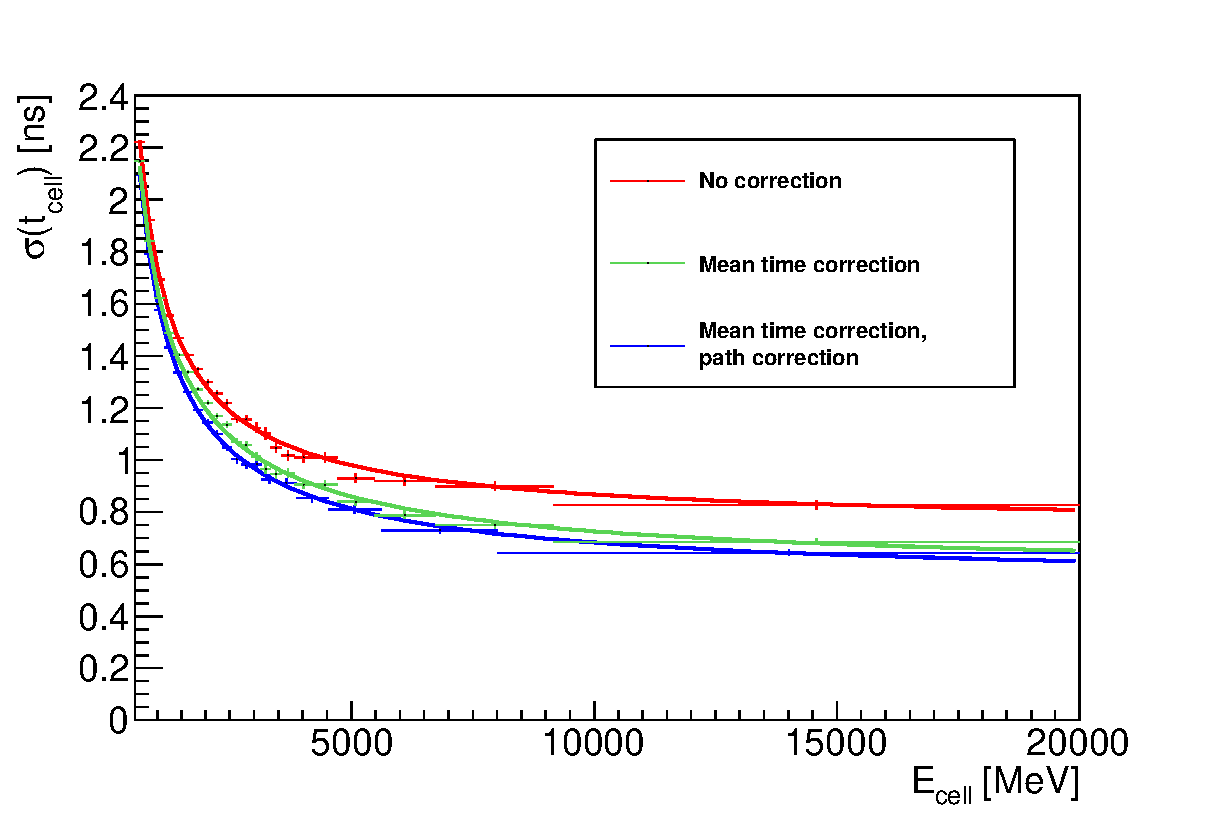
\includegraphics[width=0.8\textwidth]{TileTimingPerformance/Figures/compare_nophi.eps}
  \end{center}
  \caption{Cell time resolution as a function of energy with corrections and selections applied.}
  \label{fig:res_comp}
\end{figure}

\subsection{Open questions}
\label{sec:pileup}
After implementing the corrections, some differences among the samples remain.
Figure \ref{fig:final_split} shows the resolution and mean time dependence after the corrections.
Some differences in resolution are observed, being the D sample the one which profited most from the correction of the path and fiber length difference, as expected.

\begin{figure}[tb!]
  \begin{center}
    \begin{subfigure}{0.49\textwidth}
    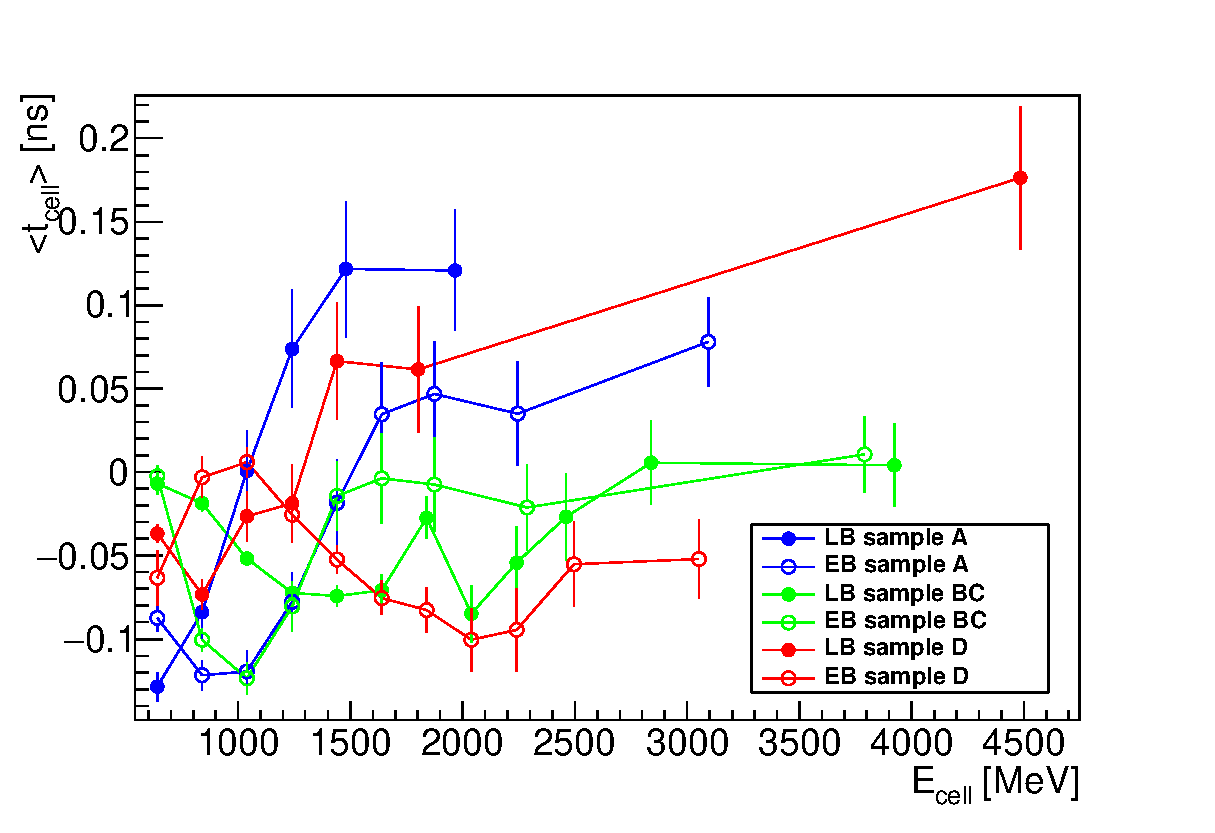
\includegraphics[width=\textwidth]{TileTimingPerformance/Figures/final_split_mean.eps}
      \caption{}
      \label{fig:final_split_mean}
    \end{subfigure}
    \begin{subfigure}{0.49\textwidth}
      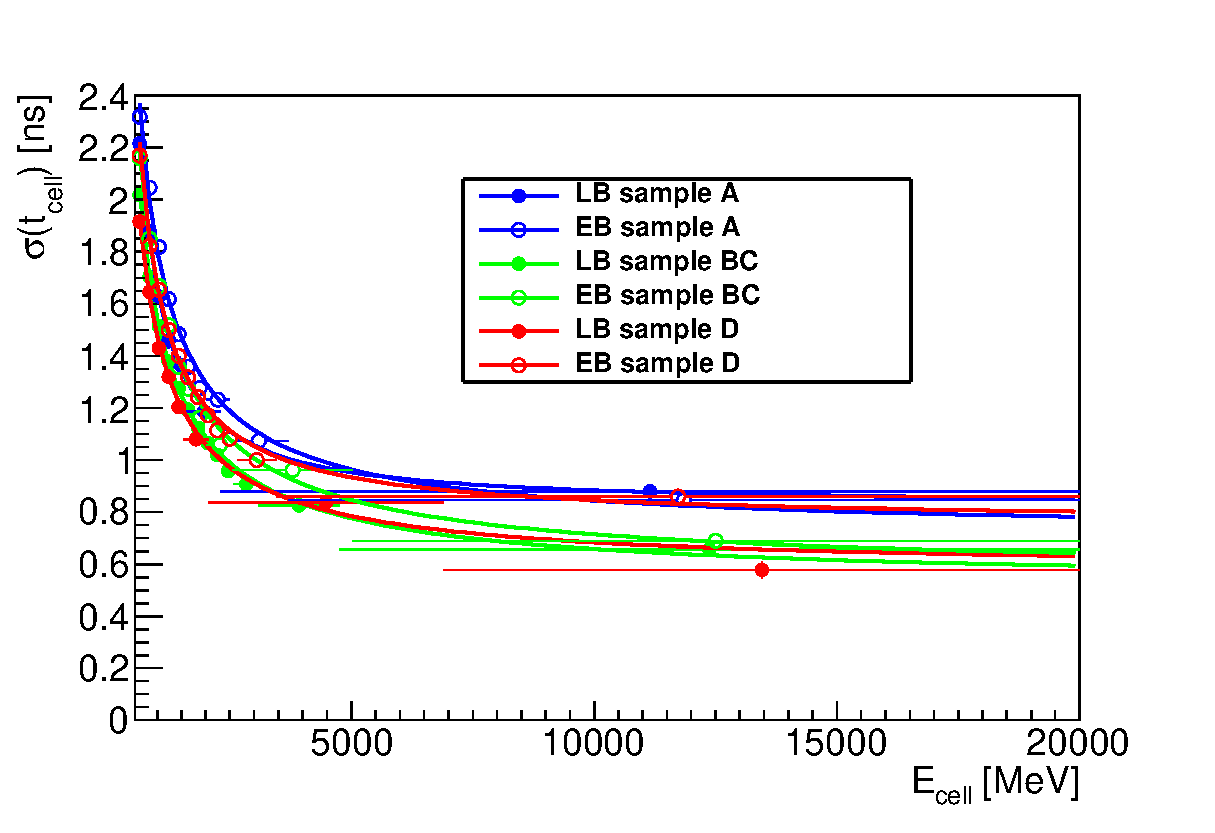
\includegraphics[width=\textwidth]{TileTimingPerformance/Figures/final_split_res.eps}
      \caption{}
      \label{fig:final_split_res}
    \end{subfigure}
  \end{center}
  \caption{(a) Mean cell time and (b) resolution dependence with energy in the individual samples after applying selections and corrections.}
  \label{fig:final_split}
\end{figure}


Table~\ref{tab:res_comp} shows the value of the resolution for each sample at \unit[850]{\mev}, ordered by resolution. The resolution is better for cells in the central region, and further away from the beam line.
One possible explanation for the difference in resolution would be the effect of \pileup.
Figure~\ref{fig:minbias} shows the distribution of the integrated current in the calorimeter~\cite{minbias}, which is an indicator of the \pileup\ presence.
It can be seen that roughly the same pattern applies, with LB sample D being the less affected by \pileup\ and EB sample A the most.
Although \pileup\ is probably one further effect on the resolution, the precise impact of this effect has not been measured.

\begin{table}
  \begin{center}
  \begin{tabular}{ c c c }
  \toprule
  \toprule
  Partition & Sample & $\sigma(t_{\rm cell})$ \\
  \midrule
  LB & D & $\unit[1.64]{ns}$ \\ 
  LB & BC & $\unit[1.71]{ns}$ \\ 
  EB & D & $\unit[1.82]{ns}$ \\ 
  EB & BC & $\unit[1.85]{ns}$ \\ 
  LB & A & $\unit[1.88]{ns}$ \\ 
  EB & A & $\unit[2.05]{ns}$ \\
  \bottomrule
  \bottomrule
\end{tabular} 
  \caption{Resolution for the different partitions and samples at an energy of \unit[850]{\mev}.}
  \label{tab:res_comp}
  \end{center}
\end{table}

\begin{figure}[tb!]
  \begin{center}
    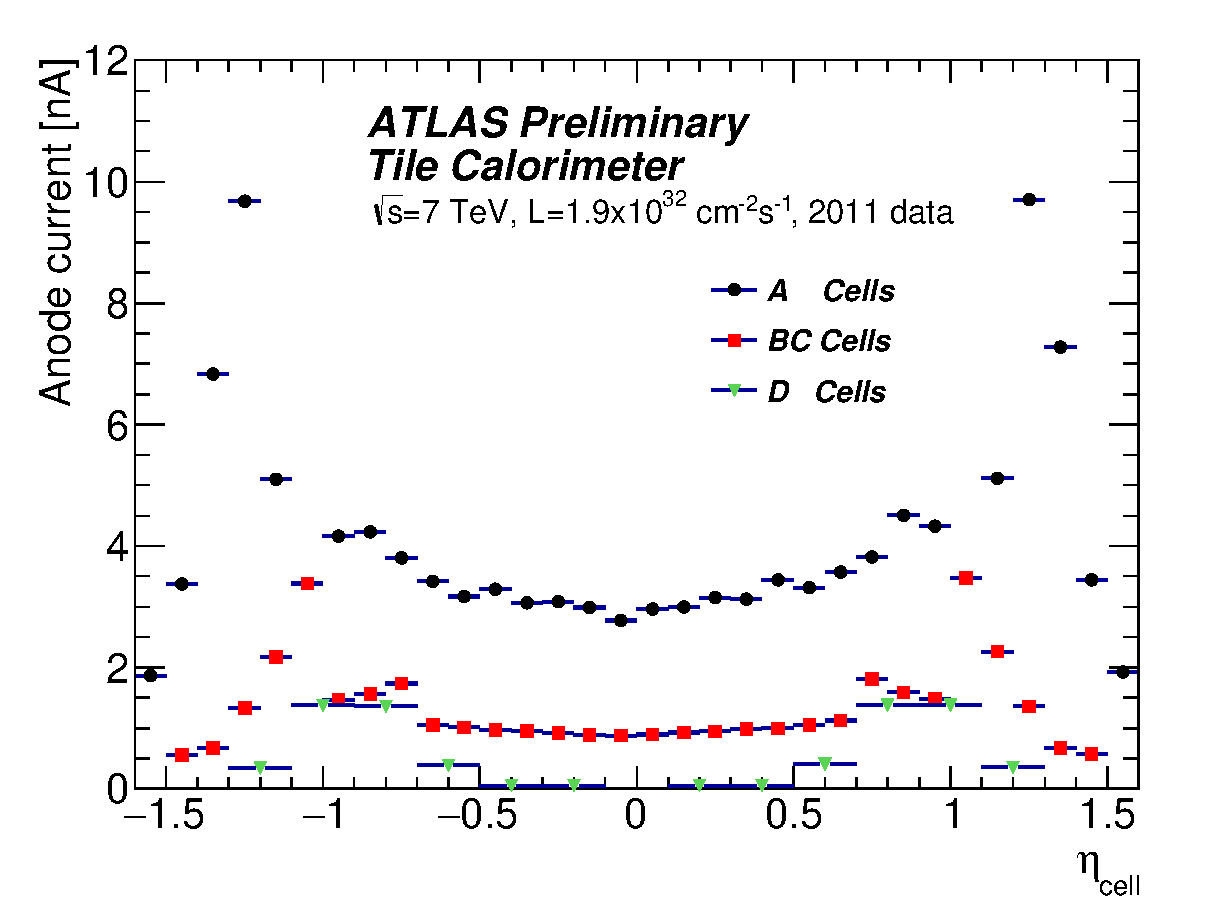
\includegraphics[width=0.6\textwidth]{TileTimingPerformance/Figures/minbias.eps}
  \end{center}
  \caption{Integrated anode current per sample as a function of the cell pseudo-rapidity. The integrated current can be regarded as a measure of the \pileup\ activity.}
  \label{fig:minbias}
\end{figure}


The difference in mean time can also probably be explained by \pileup.
The presence of \pileup\ and possible imperfections during the reconstruction and selection process can produce a small percentage of hadronic contamination of the muon sample.
The effect of this contamination can affect the kinematic regions in which the muon sample has low statistics.
Figure \ref{fig:muon_dist} shows the distribution of energy deposition in two samples.
Comparing to the mean time behavior it can be seen that an increase of the mean time can be seen in the regions with low statistics.
This can be due to the higher times measured in hadronic showers.

\begin{figure}[tb!]
  \begin{center}
    \begin{subfigure}{0.49\textwidth}
      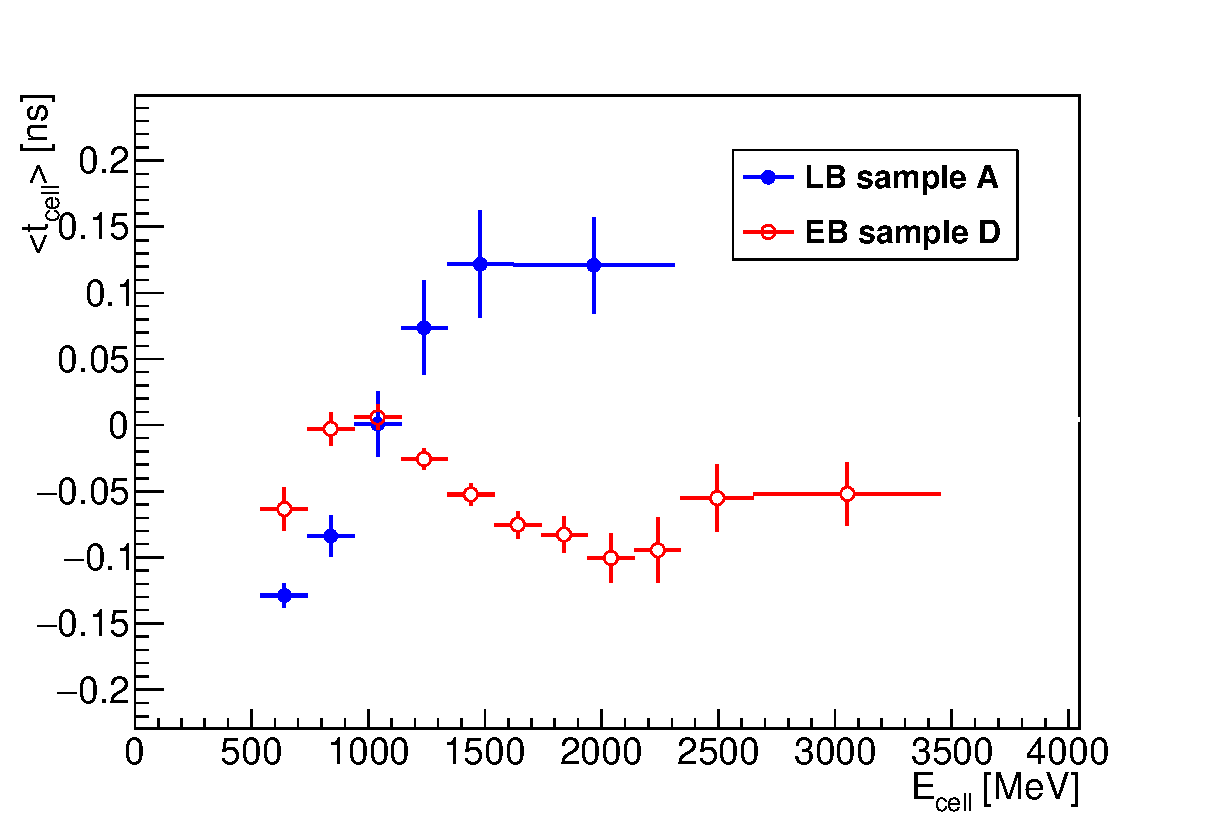
\includegraphics[width=\textwidth]{TileTimingPerformance/Figures/gmean.eps}
      \caption{}
      \label{fig:gmean}
    \end{subfigure}
    \begin{subfigure}{0.49\textwidth}
      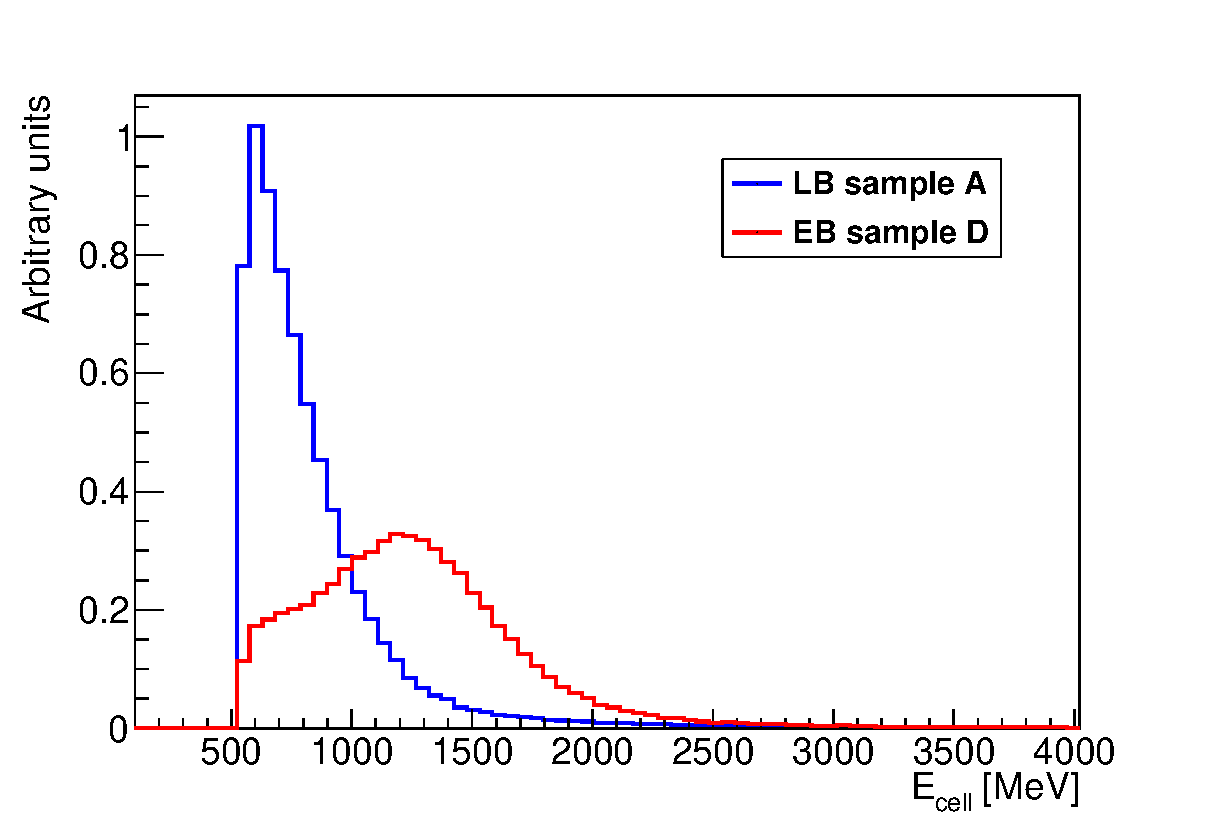
\includegraphics[width=\textwidth]{TileTimingPerformance/Figures/muondist.eps}
      \caption{}
      \label{fig:muondist}
    \end{subfigure}
  \end{center}
  \caption{(a) Mean time dependence and (b) cell energy distribution.}
  \label{fig:muon_dist}
\end{figure}

%It is worth to remember that the biggest variation of the mean time does not reach $\unit[0.5]{\sigma}$.
%Therefore the study of the mean time evolution has to be taken cautiously.

\subsection{Comparison of the timing performance}
Finally, a comparison between the performance of the time measurement
with muons and jets can be done in the high-gain
regime.
Figure~\ref{fig:public} compares the different resolution and
mean time as a function of energy for muons and hadronic showers,
after the mean cell times have been aligned separately in each analysis, 
since it has been shown that both analyses measure a different mean time.

\begin{figure}[p!]
  \begin{center}
    \begin{subfigure}{\textwidth}
      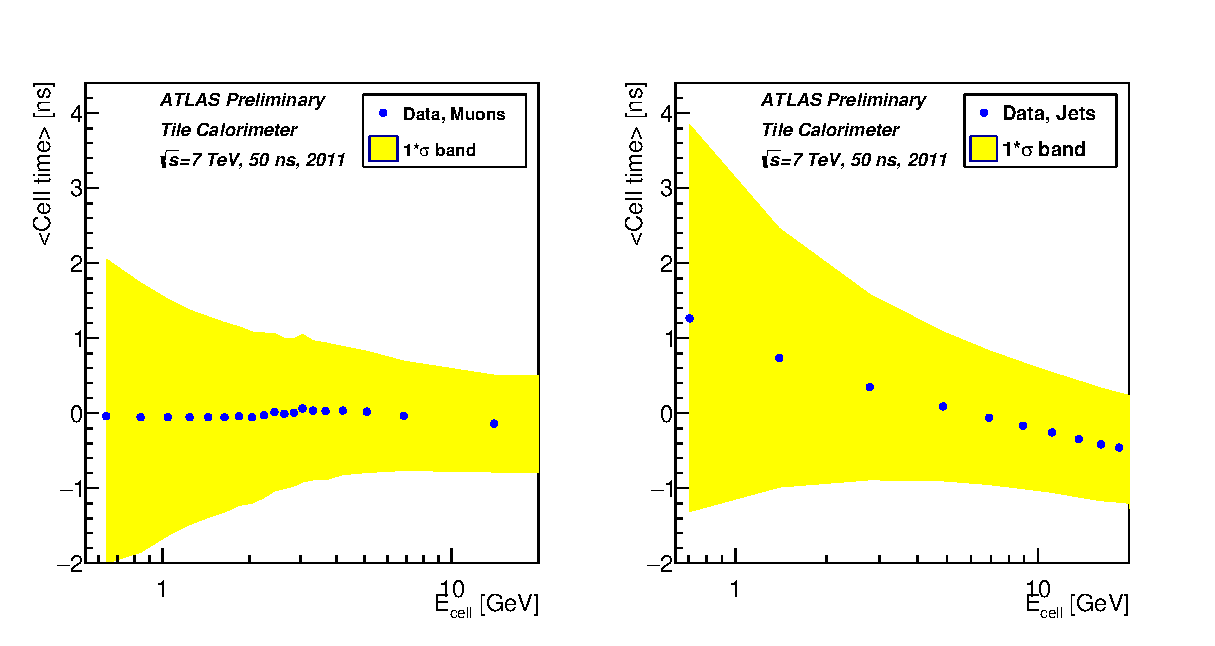
\includegraphics[width=\textwidth]{TileTimingPerformance/Figures/mean_merge.eps}
      \caption{}
      \label{fig:pub_mean}
    \end{subfigure}
    \begin{subfigure}{0.6\textwidth}
      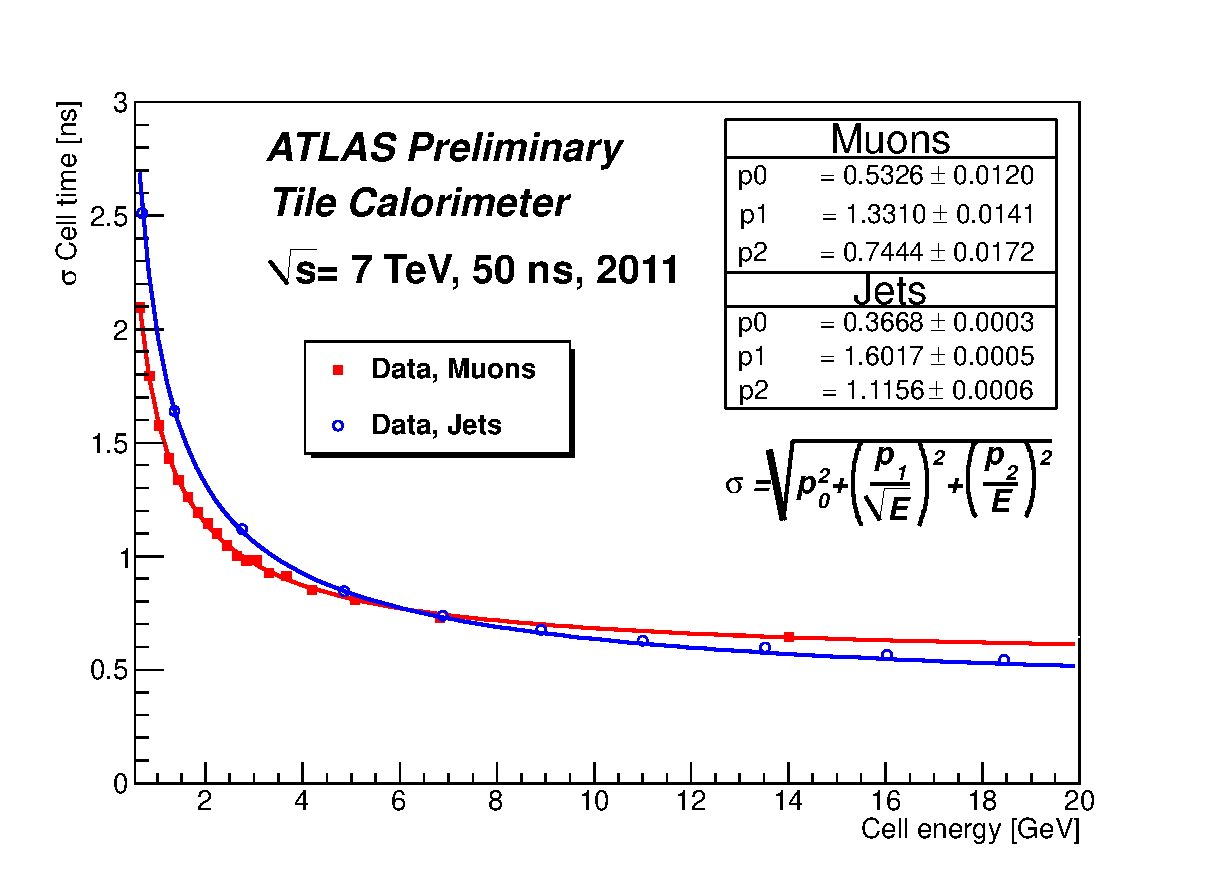
\includegraphics[width=\textwidth]{TileTimingPerformance/Figures/pub_resolution.eps}
      \caption{}
      \label{fig:pub_res}
    \end{subfigure}
  \end{center}
  \caption{(a) Mean cell time and (b) resolution  as a function of energy for muons and jets~\cite{timingpublicplots}. Slow neutrons in the hadronic showers introduce a dependence of the cell time respect to the energy. The $1\sigma$ band represent the RMS of the time distribution at a given energy.}
  \label{fig:public}
\end{figure}


The main difference is the dependence of the mean time with
energy.
The mean time of the muons stays almost constant along all the
energy range, whereas hadronic showers tend towards higher mean times
for low energies.
This is caused by the slow neutrons in
the shower, whose contribution becomes relevant at low energies.

\section{Conclusions}

The time performance of the ATLAS hadronic Tile calorimeter has been
studied with isolated muons and compared to jets from collision events.
The leading dependence of the time resolution is known to be the energy deposition in the cell.
After its measurement and parameterization, further observables are investigated in order to
fully understand the measured performance and to be able to improve it.

The main source of resolution degradation has been identified to be a 
deviation from the expected zero mean time for each cell, 
with a shift towards negative times for cells further away from the interaction point.
This effect has been studied and is caused by the use of 
jet data in the calibration of cells and in the maintenance of the database's timing constants.
%After correcting for this effect the resolution improves but the modeling of the performance as a function of energy alone remains insufficient.

Further geometrical effects were studied, such as the difference in path length for muons traversing a cell with some distance to the center.
It has been shown that this effect is non-negligible, especially for large cells, in which it can account for up to \unit[3]{ns} in arrival-time difference.
The difference in fiber length that the light has to travel in the fibers after read-out has also been taken into account.
A correction has been introduced to account for this effect, improving the resolution.

The study of these observables and the derived corrections has allowed to improve the resolution of the time measurement up to $\unit[20]{\%}$ depending on the energy range.
These corrections also significantly improve the goodness of the fit for the parameterization of the time resolution as a function of cell energy.
